\providecommand{\toplevelprefix}{../..}  %
\documentclass[../../book-main_ro.tex]{subfiles}

\begin{document}

\chapter{Metode de optimizare}
\label{app:optimization}

\begin{quote}
``{\em Deoarece construcția întregului univers este perfectă și este creată de înțelepciunea creatorului, nimic nu apare în univers în care să nu putem vedea sensul unui maxim sau minim.}''

$~$\hfill -- L. Euler
 \end{quote}
\vspace{5mm}

În acest capitol, oferim o scurtă introducere în unii dintre cei mai elementari, dar importanți algoritmi de optimizare folosiți în această carte. Scopul este doar de a ajuta cititorul să aplice acești algoritmi la problemele studiate în această carte, nu de a obține o înțelegere profundă despre acești algoritmi. Prin urmare, nu vom oferi o justificare completă pentru algoritmii introduși, în ceea ce privește garanțiile de performanță.

\section{Coborârea cea mai abruptă}


Optimizarea se ocupă cu întrebarea cum să găsim unde o funcție, să zicem $L(\theta)$, atinge valoarea sa minimă. Matematic, aceasta este enunțată ca o problemă:
\begin{equation}
    \argmin_{\theta \in \Theta} \cL(\theta),
\end{equation}
unde $\Theta$ reprezintă un domeniu la care argumentul $\x$ este limitat. Adesea (și dacă nu se menționează altfel, în acest capitol) $\Theta$ este pur și simplu $\R^n$. Fără pierderea generalității, presupunem că aici funcția $\cL(\theta)$ este netedă\footnote{În cazul în care funcția \(\cL\) nu este netedă, înlocuim gradientul său cu un așa-numit \textit{subgradient}.}.

Eficiența găsirii minimelor (globale) depinde de ce informații avem despre funcția \(\cL\). Pentru majoritatea problemelor de optimizare considerate în această carte, dimensiunea lui \(\theta\), să zicem \(n\), este foarte mare. Aceasta face ca calcularea sau accesarea informațiilor locale despre \(\ell\) să fie costisitoare. În special, deoarece gradientul \(\nabla \cL\) are \(n\) intrări, este adesea rezonabil de calculat; cu toate acestea, Hessianul \(\nabla^{2} \cL\) are \(n^{2}\) intrări, ceea ce este adesea extrem de nepractic de calculat (și același lucru este valabil pentru derivatele de ordin superior). Prin urmare, este tipic să presupunem că avem informația de ordin zero, adică suntem capabili să evaluăm \(\cL(\theta)\), și informația de prim ordin, adică suntem capabili să evaluăm \(\nabla \cL(\theta)\). Teoreticienii optimizării pot reformula aceasta spunând că avem un ``oracol de \textit{prim ordin}''. Toți algoritmii de optimizare pe care îi introducem în această secțiune folosesc doar un oracol de prim ordin.\footnote{Trimitem cititorii la cartea de \cite{Wright-Ma-2022} pentru o introducere mai sistematică în algoritmii de optimizare într-un spațiu de dimensiune mare, inclusiv algoritmi care presupun oracole de ordin superior.}

\subsection{Coborârea gradientului vanilla pentru probleme netede}

Cea mai simplă și mai utilizată metodă pentru optimizare este \textit{coborârea gradientului} (GD). A fost introdusă pentru prima dată de Cauchy în 1847. Ideea este foarte simplă: pornind de la o stare inițială, facem pași mici iterativ astfel încât fiecare pas să reducă valoarea funcției $\cL(\theta)$.

Să presupunem că starea curentă este $\theta$. Vrem să facem un pas mic, să zicem de distanță $h$, într-o direcție, indicată de un vector $\vv$, pentru a ajunge la o nouă stare $\theta + h\vv$ astfel încât valoarea funcției să scadă:
\begin{equation}
    \cL(\theta + h\vv) \leq \cL(\theta).
\end{equation}
Pentru a găsi o astfel de direcție $\vv$, putem aproxima $\cL(\theta + h\vv)$ printr-o expansiune Taylor în jurul lui \(h = 0\):
\begin{equation}
    \cL(\theta + h\vv) = \cL(\theta) + h\ip{\nabla \cL(\theta)}{\vv} + o(h),
\end{equation}
unde produsul scalar aici (și în acest capitol) va fi produsul scalar \(\ell^{2}\), adică \(\ip{\vx}{\vy} = \vx^{\top}\vy\). Pentru a găsi direcția de \textit{coborâre cea mai abruptă}, încercăm să minimizăm această expansiune Taylor printre vectorii unitari \(\vv\). Dacă \(\nabla \cL(\theta) = \vzero\), atunci al doilea termen de mai sus este \(0\) indiferent de valoarea lui \(\vv\), deci nu putem încerca să facem progrese, adică algoritmul a conversat. Pe de altă parte, dacă \(\nabla \cL(\theta) \neq \vzero\) atunci este valabil
\begin{equation}\label{eq:steepest_descent_l2_norm}
    \argmin_{\substack{\vv \in \R^{d} \\ \norm{\vv}_{2} = 1}} [\cL(\theta) + h\ip{\nabla \cL(\theta)}{\vv}] = \argmin_{\substack{\vv \in \R^{d} \\ \norm{\vv}_{2} = 1}} \ip{\nabla \cL(\theta)}{\vv} = -\frac{\nabla \cL(\theta)}{\norm{\nabla \cL(\theta)}_{2}},
\end{equation}
Cu alte cuvinte, aceasta înseamnă că valoarea lui \(\cL(\theta + h\vv)\) scade cel mai rapid de-a lungul direcției \(\vv = -\nabla \cL(\theta) / \norm{\nabla \cL(\theta)}_{2}\), pentru \(h\) suficient de mic. Aceasta conduce la metoda coborârii gradientului: Din starea curentă $\theta_k$ ($k=0, 1, \ldots$), facem un pas de mărime $h$ în direcția gradientului negativ pentru a ajunge la următoarea iterație,
\begin{equation}
    \theta_{k+1} = \theta_k - h \nabla \cL(\theta_k). 
\end{equation}
Mărimea pasului \(h\) este numită și \textit{rata de învățare} în contextele de învățare automată.

\subsubsection{Selecția mărimii pasului}

Întrebarea rămasă este care ar trebui să fie mărimea pasului $h$? Dacă alegem $h$ să fie prea mic, valoarea funcției poate scădea foarte încet, așa cum se arată în graficul din mijloc din \Cref{fig:step-size}. Dacă $h$ este prea mare, valoarea ar putea să nici nu scadă deloc, așa cum se arată în graficul din dreapta din \Cref{fig:step-size}.

\begin{figure}[h]
    \centering
    \includegraphics[height=3.5cm]{\toplevelprefix/chapters/appendixA/figs/GD-1.png}
    \hspace{3mm}
    \includegraphics[height=3.5cm]{\toplevelprefix/chapters/appendixA/figs/GD-2.png}
    \hspace{3mm}
    \includegraphics[height=3.5cm]{\toplevelprefix/chapters/appendixA/figs/GD-3.png}
    \caption{Efectul mărimii pasului $h$ asupra convergenței metodei coborârii gradientului.}
    \label{fig:step-size}
\end{figure}

Deci mărimea pasului $h$ ar trebui aleasă pe baza peisajului funcției $\cL(\theta_k)$. Ideal, pentru a alege cea mai bună mărime a pasului $h$, putem rezolva următoarea problemă de optimizare peste o singură variabilă $h$:
\begin{equation}
    h = \argmin_{h\geq 0} \cL(\theta_k - h\nabla \cL(\theta_k)).
\end{equation}
Această metodă de alegere a mărimii pasului se numește \textit{căutare pe linie}. Cu toate acestea, când funcția $L(\theta_k)$ este complicată, ceea ce este de obicei cazul pentru antrenarea unei rețele neuronale profunde, această optimizare unidimensională este foarte dificil de rezolvat la fiecare iterație a coborârii gradientului.

Atunci cum ar trebui să alegem o mărime adecvată a pasului $h$? O abordare comună și clasică este să încercăm să obținem o bună aproximare a peisajului local în jurul stării curente $\theta$ pe baza unor cunoștințe despre peisajul general al funcției $\cL(\theta)$.

\begin{figure}
    \centering 
    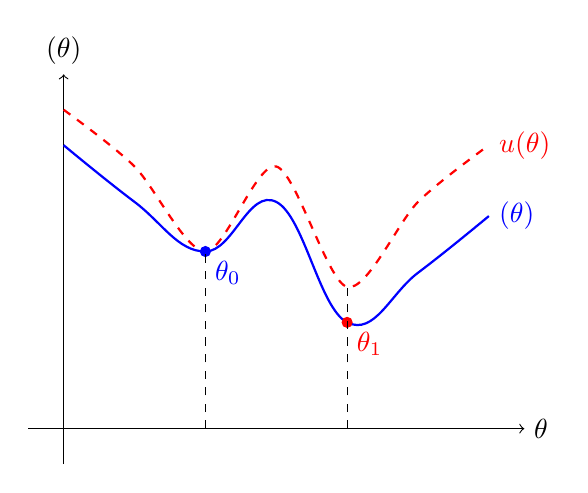
\begin{tikzpicture}[scale=0.9]
        \draw[->] (-0.5,0) -- (6.5,0) node[right] {$\theta$};
        \draw[->] (0,-0.5) -- (0,5) node[above] {$\cL(\theta)$};
        
        \draw[thick, blue] plot[smooth, tension=0.7] coordinates {
            (0,4) (1,3.2) (2,2.5) (3,3.2) (4,1.5) (5,2.2) (6,3)
        } node[right] {$\cL(\theta)$};
        
        \draw[thick, red, dashed] plot[smooth, tension=0.5] coordinates {
            (0,4.5) (1,3.7) (2,2.5) (3,3.7) (4,2) (5,3.2) (6,4)
        } node[right] {$u(\theta)$};
        
        \filldraw[blue] (2,2.5) circle (2pt) node[below right] {$\theta_0$};
        
        \filldraw[red] (4,1.5) circle (2pt) node[below right] {$\theta_1$};
        
        \draw[dashed] (2,0) -- (2,2.5);
        \draw[dashed] (4,0) -- (4,2);
    \end{tikzpicture}
    \caption{\small\textbf{Schema și intuiția majorizării-minimizării.} O funcție \(\cL \colon \Theta \to \R\) are o limită superioară globală \(u \colon \Theta \to \R\) care întâlnește \(L\) în cel puțin un punct \(\theta_{0}\). Apoi, găsirea lui \(\theta_{1}\) care minimizează \(u\) va îmbunătăți valoarea lui \(\cL\) de la \(\cL(\theta_{0})\). Rețineți că rezultate similare pot fi arătate despre limitele superioare locale.}
    \label{fig:majorization_minimization}
\end{figure}

Condițiile comune pentru peisajul lui \(\cL(\theta)\) includ:
\begin{itemize}
    \item \(\alpha\)-Convexitate puternică. Reamintim că \(\cL\) este \textit{\(\alpha\)-puternic convexă} dacă graficul său se află deasupra unei limite inferioare pătratice globale de pantă \(\alpha\), adică,
    \begin{equation}
        \cL(\theta) \geq l_{\theta_{0}, \alpha}(\theta) \doteq \cL(\theta_{0}) + \ip{\nabla \cL(\theta_{0})}{\theta - \theta_{0}} + \frac{\alpha}{2}\norm{\theta - \theta_{0}}_{2}^{2}
    \end{equation}
    pentru orice ``punct de bază'' \(\theta_{0}\). Spunem că \(\cL\) este \textit{convexă} dacă este \(0\)-puternic convexă, adică graficul său se află deasupra tangentelor sale. Este ușor de arătat (demonstrația ca exercițiu) că funcțiile puternic convexe au minime globale unice. Un alt fapt important (demonstrația ca exercițiu) este că funcțiile \(\alpha\)-puternic convexe de două ori diferențiabile \(\cL\) au Hessiene (simetrice) \(\nabla^{2}\cL\) a căror valoare proprie minimă este \(\geq \alpha\). Pentru \(\alpha > 0\) aceasta implică că Hessianul este simetric pozitiv definit, iar pentru \(\alpha = 0\) (adică \(\cL\) este convexă) aceasta implică că Hessianul este simetric pozitiv semidefinit.
    \item \(\beta\)-Gradient Lipschitz (numit și \(\beta\)-Netezime). Reamintim că \(\cL\) are \textit{\(\beta\)-gradient Lipschitz} dacă \(\nabla \cL\) există și este \(\beta\)-Lipschitz, adică,
    \begin{equation}
        \norm{\nabla \cL(\theta) - \nabla \cL(\theta_{0})}_{2} \leq \beta \norm{\theta - \theta_{0}}_{2}.
    \end{equation}
    pentru orice ``punct de bază'' \(\theta_{0}\). Este ușor de arătat (demonstrația ca exercițiu) că aceasta este echivalentă cu \(\cL\) având o limită superioară pătratică globală de pantă \(\beta\), adică,
    \begin{equation}
        \cL(\theta) \leq u_{\theta_{0}, \beta}(\theta) \doteq \cL(\theta_{0}) + \ip{\nabla \cL(\theta_{0})}{\theta - \theta_{0}} + \frac{\beta}{2}\norm{\theta - \theta_{0}}_{2}^{2}.
    \end{equation}
    pentru orice ``punct de bază'' \(\theta_{0}\). Un alt fapt important (demonstrația ca exercițiu) este că funcțiile convexe cu \(\beta\)-gradient Lipschitz de două ori diferențiabile au Hessiene (simetrice) \(\nabla^{2}\cL\) a căror valoare proprie cea mai mare este \(\leq \beta\).
\end{itemize}
Mai întâi, să presupunem că \(\cL\) are \(\beta\)-gradient Lipschitz (dar nu este neapărat chiar convexă). Vom folosi această ocazie pentru a introduce o temă comună de optimizare: \textit{pentru a minimiza \(\cL\), putem minimiza o limită superioară pe \(L\)}, care este justificată de următoarea lemă vizualizată în \Cref{fig:majorization_minimization}.
\begin{lemma}[Majorizare-Minimizare]\label{lem:majorization_minimization}
    Să presupunem că \(u \colon \Theta \to \R\) este o limită superioară globală pe \(\cL\), și anume \(\cL(\theta) \leq u(\theta)\) pentru toți \(\theta \in \Theta\). Să presupunem că se întâlnesc cu egalitate la \(\theta_{0}\), adică \(\cL(\theta_{0}) = u(\theta_{0})\). Atunci
    \begin{equation}
        \theta_{1} \in \argmin_{\theta \in \Theta}u(\theta) \implies \cL(\theta_{1}) \leq u(\theta_{1}) \leq u(\theta_{0}) = \cL(\theta_{0}).
    \end{equation}
\end{lemma}

Vom folosi această lemă pentru a arăta că putem folosi proprietatea gradientului Lipschitz pentru a ne asigura că fiecare pas de gradient nu poate înrăutăți valoarea lui \(\cL\). Într-adevăr, la fiecare punct de bază \(\theta_{0}\), avem că \(u_{\theta_{0}, \beta}\) este o limită superioară globală pe \(\cL\), și \(u_{\theta_{0}, \beta}(\theta_{0}) = \cL(\theta_{0})\). Prin urmare, prin \Cref{lem:majorization_minimization}
\begin{equation}
    \text{dacă \(\theta\) minimizează \(u_{\theta_{0}, \beta}\) atunci} \quad \cL(\theta) \leq u_{\theta_{0}, \beta}(\theta) \leq u_{\theta_{0}, \beta}(\theta_{0}) = \cL(\theta_{0}).
\end{equation}
Aceasta ne motivează, când găsim o actualizare pentru a obține \(\theta_{k + 1}\) din \(\theta_{k}\), putem în schimb să minimizăm limita superioară \(u_{\theta_{k}, \beta}\) peste \(\theta\) și să setăm aceasta să fie \(\theta_{k + 1}\). Prin minimizarea \(u_{\theta_{k}, \beta}\) (demonstrația ca exercițiu) obținem
\begin{equation}\label{eq:GD}
    \theta_{k + 1} = \theta_{k} - \frac{1}{\beta}\nabla \cL(\theta_{k}) \implies \cL(\theta_{k + 1}) \leq \cL(\theta_{k}).
\end{equation}
Aceasta implică că o mărime a pasului \(h = 1/\beta\) este o rată de învățare utilizabilă, dar nu oferă o rată de convergență sau nu certifică că \(L(\theta_{k})\) converge de fapt la \(\min_{\theta}\cL(\theta)\). Aceasta necesită puțin mai multă rigoare, pe care o urmărim acum.

Acum, să presupunem că \(\cL\) este \(\alpha\)-puternic convexă, are \(\beta\)-gradient Lipschitz și are optimul global \(\theta^{\star}\). Vom arăta că \(\theta_{k}\) va converge direct la optimul global unic \(\theta^{\star}\), care este o formă foarte puternică de convergență. În special, vom limita \(\norm{\theta^{\star} - \theta_{k}}_{2}\) folosind atât convexitatea puternică, cât și caracterul Lipschitz al gradientului lui \(\cL\), adică privind vecinătatea în jurul lui \(\theta_{k}\):\footnote{În această demonstrație, pasul de invocare a \(\beta\)-Gradientului Lipschitz este puțin non-trivial. Lăsăm și acest pas ca exercițiu, cu indiciul de a înlocui \(\theta = \theta_{0} - h\nabla \cL(\theta_{0})\) în identitatea gradientului Lipschitz.}
\begin{align}
    \norm{\theta^{\star} - \theta_{k + 1}}_{2}^{2}
    &\leq \norm{\theta^{\star} - \theta_{k} + h\nabla \cL(\theta_{k})}_{2}^{2} \\ 
    &= \norm{\theta^{\star} - \theta_{k}}_{2}^{2} + 2h\ip{\nabla \cL(\theta_{k})}{\theta^{\star} - \theta_{k}} + h^{2}\norm{\nabla \cL(\theta_{k})}_{2}^{2} \\ 
    &\leq \norm{\theta^{\star} - \theta_{k}}_{2}^{2} + 2h\bp{\cL(\theta^{\star}) - \cL(\theta_{k}) - \frac{\alpha}{2}\norm{\theta^{\star} - \theta_{k}}_{2}^{2}} + h^{2}\norm{\nabla \cL(\theta_{k})}_{2}^{2} \quad \text{(\(\alpha\)-SC)} \\
    &= \bp{1 - \alpha h}\norm{\theta^{\star} - \theta_{k}}_{2}^{2} + 2h(\cL(\theta^{\star}) - L(\theta_{k})) + h^{2}\norm{\nabla \cL(\theta_{k})}_{2}^{2} \\
    &\leq \bp{1 - \alpha h}\norm{\theta^{\star} - \theta_{k}}_{2}^{2} + 2h(\cL(\theta^{k}) - \cL(\theta^{\star})) + 2h^{2}\beta(\cL(\theta_{k}) - \cL(\theta^{\star})) \quad \text{(\(\beta\)-LG)} \\
    &= \bp{1 - \alpha h}\norm{\theta^{\star} - \theta_{k}}_{2}^{2} - 2h(1 - \beta h)(\cL(\theta_{k}) - \cL(\theta^{\star})).
\end{align}
Pentru a ne asigura că iterația coborârii gradientului face progrese, trebuie să alegem mărimea pasului astfel încât \(1 - \beta h \geq 0\), adică \(h \leq 1/\beta\). Dacă apare o astfel de setare, atunci
\begin{align}
    \norm{\theta^{\star} - \theta_{k + 1}}_{2}^{2} 
    &\leq (1 - \alpha h)\norm{\theta^{\star} - \theta_{k}}_{2}^{2} \leq (1 - \alpha h)^{2}\norm{\theta^{\star} - \theta_{k - 1}}_{2}^{2} \leq \cdots \\ 
    &\leq (1 - \alpha h)^{k + 1}\norm{\theta^{\star} - \theta_{0}}_{2}^{2}.
\end{align}
Pentru a minimiza partea dreaptă, putem seta \(h = 1/\beta\), ceea ce obține
\begin{equation}
    \norm{\theta^{\star} - \theta_{k + 1}}_{2}^{2} \leq (1 - \alpha/\beta)^{k + 1}\norm{\theta^{\star} - \theta_{0}}_{2}^{2},
\end{equation}
arătând convergența la optimul global cu eroare care scade exponențial. Observați că aici am folosit o rată de convergență pentru a obține o \textit{mărime favorabilă a pasului} de \(h = 1/\beta\). Acest motiv va reapărea în această secțiune.

Încheiem această secțiune cu o avertizare: învățarea unui optim global este (de obicei) impracticabil de dificilă. În anumite condiții, putem asigura că iterațiile coborârii gradientului converg la un \textit{optim local}. De asemenea, în condiții mai relaxate, putem asigura convergența \textit{locală}, adică că iterațiile converg la un optim (global sau local) dacă secvența este inițializată suficient de aproape de optim.



\subsection{Coborârea gradientului precondiționată pentru probleme prost condiționate}


\begin{figure}
    \includegraphics[width=\textwidth]{\toplevelprefix/chapters/appendixA/figs/hessian_geometry.png}
    \caption{\small\textbf{Gradientul negativ \(-\nabla \cL_{\lambda}\) și câmpul vectorial precondiționat (pasul metodei lui Newton) \(-[\nabla^{2}\cL_{\lambda}]^{-1}[\nabla \cL_{\lambda}]\)} unde \(\lambda = 19\). Există o secțiune a spațiului unde urmarea câmpului vectorial gradient negativ face foarte puține progrese către găsirea minimului, dar în toate cazurile urmarea câmpului vectorial al metodei lui Newton obține viteză egală de progres către optim, deoarece gradientul este albit. Deoarece Hessianul aici este diagonal, algoritmii de rată de învățare adaptivă (de exemplu, Adam, așa cum va fi discutat mai târziu în secțiune) pot face progrese similare cu metoda lui Newton, dar un Hessian ne-aliniat pe axe poate chiar împiedica Adam să reușească rapid.}
    \label{fig:hessian_geometry}
\end{figure}

\subsubsection{Metoda lui Newton}

Există unele probleme netede și probleme puternic convexe pe care coborârea gradientului totuși funcționează destul de prost. De exemplu, fie \(\lambda \geq 0\) și fie \(\cL_{\lambda} \colon \R^{2} \to \R\) de forma
\begin{equation}
    \cL_{\lambda}(\theta) = \cL_{\lambda}\rp{\mat{\theta_{1} \\ \theta_{2}}} \doteq \frac{1}{2}\bc{(1 + \lambda) \theta_{1}^{2} + \theta_{2}^{2}} = \frac{1}{2}\theta^{\top}\mat{1 + \lambda & 0 \\ 0 & 1}\theta.
\end{equation}
Această problemă este \(1\)-puternic convexă și are \((1 + \lambda)\)-gradient Lipschitz. Rata de convergență este apoi geometrică cu rata \(1 - 1/(1 + \lambda)\). Pentru \(\lambda\) mare, aceasta încă nu este foarte rapidă. În această secțiune, vom introduce o clasă de probleme de optimizare care pot optimiza cu succes astfel de funcții prost condiționate.

Cheia se află în \textit{curbura} obiectivului, care este dată de Hessian. Să presupunem că (ca un contrafactual) am avea un oracol de \textit{ordinul doi} care ne-ar permite să calculăm \(\cL(\theta)\), \(\nabla \cL(\theta)\) și \(\nabla^{2}\cL(\theta)\). Apoi, în loc să alegem o direcție de coborâre \(\vv\) pentru a optimiza expansiunea Taylor de ordinul întâi în jurul lui \(\theta\), am putea optimiza în schimb expansiunea Taylor de ordinul doi. Intuitiv, aceasta ne-ar permite să încorporăm informații despre curbură în actualizare.

Să efectuăm acest calcul. Expansiunea Taylor de ordinul doi a lui \(\cL(\theta + h\vv)\) în jurul lui \(h = 0\) este
\begin{equation}
    \cL(\theta + h\vv) = \cL(\theta) + h\ip{\nabla \cL(\theta)}{\vv} + \frac{1}{2}h^{2}\ip{[\nabla^{2}\cL(\theta)]\vv}{\vv} + o(h^{2}).
\end{equation}
Apoi putem calcula direcția de coborâre:
\begin{align}
    \argmin_{\substack{\vv \in \R^{n} \\ \norm{\vv}_{2} = 1}}\bs{\cL(\theta) + h\ip{\nabla \cL(\theta)}{\vv} + \frac{1}{2}h^{2}\ip{[\nabla^{2}\cL(\theta)]\vv}{\vv}} 
    &= \argmin_{\substack{\vv \in \R^{n} \\ \norm{\vv}_{2} = 1}}\bs{\ip{\nabla \cL(\theta)}{\vv} + \frac{1}{2}h\ip{[\nabla^{2}\cL(\theta)]\vv}{\vv}}.
\end{align}
Această problemă de optimizare este puțin dificil de rezolvat din cauza constrângerii \(\norm{\vv}_{2} = 1\). Dar în practică nu normalizăm niciodată direcția de coborâre \(\vv\) și folosim mărimea pasului \(h\) pentru a controla mărimea actualizării. Deci, să rezolvăm problema de mai sus peste toți vectorii \(\vv \in \R^{n}\):\footnote{Dacă \(\nabla^{2}\cL(\theta)\) nu este inversabil, atunci putem înlocui \([\nabla^{2}\cL(\theta)]^{-1}\) cu pseudoinversa Moore-Penrose a lui \(\nabla^{2}\cL(\theta)\).}
\begin{equation}
    \argmin_{\vv \in \R^{n}}\bs{\ip{\nabla \cL(\theta)}{\vv} + \frac{1}{2}h\ip{[\nabla^{2}\cL(\theta)]\vv}{\vv}} = -\frac{1}{h}[\nabla^{2}\cL(\theta)]^{-1}[\nabla \cL(\theta)].
\end{equation}
Putem astfel folosi iterația de coborâre cea mai abruptă
\begin{equation}
    \theta_{k + 1} = \theta_{k} - [\nabla^{2}\cL(\theta_{k})]^{-1}[\nabla \cL(\theta_{k})],
\end{equation}
(aceasta este celebra \textit{metodă a lui Newton}), sau
\begin{equation}
    \theta_{k + 1} = \theta_{k} - h[\nabla^{2}\cL(\theta_{k})]^{-1}[\nabla \cL(\theta_{k})],
\end{equation}
(care se numește \textit{metoda lui Newton subamortizată}). Deoarece pătratică de ordinul doi \(\cL_{\lambda}\) este egală cu expansiunea sa Taylor de ordinul doi, dacă rulăm metoda lui Newton pentru \textit{un pas}, vom obține minimul global într-\textit{un pas}, indiferent cât de mare este \(\lambda\). \Cref{fig:hessian_geometry} oferă o oarecare intuiție despre funcțiile prost condiționate și pașii de gradient versus pașii lui Newton.

\subsubsection{PGD}

În practică, \textit{nu} avem un oracol de ordinul doi care ne permite să calculăm \(\nabla^{2}\cL(\theta)\). În schimb, putem încerca să \textit{învățăm o aproximare la acesta} alături de actualizarea parametrului \(\theta_{k + 1}\) din \(\theta_{k}\).

Cum învățăm o aproximare la acesta? Vom găsi câteva ecuații pe care le satisface inversa Hessianului și apoi vom încerca să actualizăm aproximarea noastră astfel încât să satisfacă ecuațiile. Mai exact, luând seria Taylor a lui \(\nabla \cL(\theta + \delta_{\theta})\) în jurul punctului \(\theta\), obținem
\begin{equation}
    \underbrace{\nabla L(\theta + \delta_{\theta}) - \nabla \cL(\theta)}_{\doteq \delta_{\vg}} = [\nabla^{2} \cL(\theta)]\delta_{\theta} + o(\norm{\delta_{\theta}}_{2}).
\end{equation}
În acest caz avem
\begin{equation}
    \delta_{\vg} \approx [\nabla^{2}\cL(\theta)]\delta_{\theta} \implies \delta_{\theta} \approx [\nabla^{2}\cL(\theta)]^{-1}\delta_{\vg}
\end{equation}
Putem acum încerca să învățăm un precondiționator simetric pozitiv semidefinit \(P \in \R^{n \times n}\) astfel încât
\begin{equation}
    \delta_{\theta} \approx P\delta_{\vg},
\end{equation}
actualizându-l la fiecare iterație împreună cu \(\theta_{k}\). Mai exact, avem iterația \textit{PSGD}
\begin{align}
    P_{k}
    &= \mathrm{PreconditionerUpdate}(P_{k - 1}; \theta_{k}, \nabla \cL(\theta_{k})) \\ 
    \theta_{k + 1}
    &= \theta_{k} - hP_{k}\nabla \cL(\theta_{k}).
\end{align}
Această actualizare are două probleme: cum putem chiar folosi \(P\) (deoarece am spus deja că nu putem stoca o matrice \(n \times n\)) și cum putem \textit{actualiza} \(P\) la fiecare iterație? Răspunsurile sunt foarte legate; nu putem niciodată materializa \(P\) în memoria computerului, dar îl putem reprezenta folosind o factorizare de rang mic (sau metode comparabile precum \textit{factorizarea Kronecker} care este deosebit de potrivită pentru forma rețelelor neuronale profunde). Apoi pasul de actualizare a precondiționatorului este proiectat pentru a exploata structura reprezentării precondiționatorului.

Încheiem această subsecțiune cu o avertizare: în învățarea profundă, de exemplu, \(\cL\) nu este o funcție convexă și astfel metoda lui Newton (și aproximările la ea) nu au sens. În acest caz ne uităm la intuiția geometrică a metodei lui Newton pe funcții convexe, să zicem din \Cref{fig:hessian_geometry}: Hessianul invers \textit{albește} gradienții. Astfel, în loc de un precondiționator care aproximează Hessianul, putem ajusta procedurile de mai sus pentru a învăța o transformare de albire mai generală pentru gradient. Aceasta este ideea din spatele propunerii originale a PSGD \cite{li2017preconditioned}, care conține mai multe informații despre cum să stocăm și să actualizăm precondiționatorul, și optimizatori mai moderni precum Muon \cite{liu2025muon}.


\subsection{Coborârea gradientului proximal pentru probleme ne-netede}\label{subsec:pgd}

Chiar și în probleme foarte simple, cum ar fi LASSO sau învățarea de dicționar, problema nu este puternic convexă, ci doar convexă, iar obiectivul nu mai este doar neted, ci suma unei funcții netede și a unui regularizator ne-neted (cum ar fi norma \(\ell^{1}\)). Astfel de probleme sunt rezolvate de \textit{algoritmi de optimizare proximală}, care generalizează coborârea cea mai abruptă la obiective ne-netede.

Formal, să spunem că
\begin{equation}
    \cL(\theta) \doteq \cS(\theta) + \cR(\theta)
\end{equation}
unde \(\cS\) este netedă, să zicem cu \(\beta\)-gradient Lipschitz, și \(\cR\) este ne-netedă (adică aspră). Algoritmul de gradient proximal generalizează algoritmul de coborâre cea mai abruptă, folosind cadrul de majorizare-minimizare (adică \Cref{lem:majorization_minimization}) cu o limită superioară globală diferită. Mai exact, construim o astfel de limită superioară întrebând: ce se întâmplă dacă luăm limita superioară a gradientului Lipschitz a lui \(S\) dar \textit{lăsăm \(R\) în pace}? Mai exact, avem
\begin{equation}
    \cL(\theta_{1}) = \cS(\theta_{1}) + \cR(\theta_{1}) \leq u_{\theta_{0}, \beta}(\theta_{1}) \doteq \cS(\theta_{0}) + \ip{\nabla \cS(\theta_{0})}{\theta_{1} - \theta_{0}} + \frac{\beta}{2}\norm{\theta_{1} - \theta_{0}}_{2}^{2} + \cR(\theta_{1}).
\end{equation}
Rețineți că (demonstrație ca exercițiu)
\begin{equation}
    \argmin_{\theta_{1}}u_{\theta_{0}, \beta}(\theta_{1}) = \argmin_{\theta_{1}}\bs{\frac{\beta}{2}\norm*{\theta_{1} - \bp{\theta_{0} - \frac{1}{\beta}\nabla \cS(\theta_{0})}}_{2}^{2} + \cR(\theta_{1})}.
\end{equation}
Acum, dacă încercăm să minimizăm limita superioară \(u_{\theta_{0}, \beta}\), alegem un \(\theta_{1}\) care:
\begin{itemize}
    \item este aproape de actualizarea gradientului \(\theta_{0} - \frac{1}{\beta}\nabla \cS(\theta_{0})\);
    \item are o valoare mică a regularizatorului \(\cR(\theta_{1})\)
\end{itemize}
și face un compromis între aceste proprietăți în funcție de parametrul de netezime \(\beta\). În consecință, să definim operatorul proximal
\begin{equation}
    \prox_{h, \cR}(\theta) \doteq \argmin_{\theta_{1}}\bs{\frac{1}{2h}\norm{\theta_{1} - \theta}_{2}^{2} + \cR(\theta)}.
\end{equation}
Apoi, putem defini iterația \textit{coborârii gradientului proximal} care, la fiecare iterație, minimizează limita superioară \(u_{\theta_{k}, h^{-1}}\), adică,
\begin{equation}
    \theta_{k + 1} = \prox_{h, \cR}(\theta_{k} - h\nabla \cS(\theta_{k})).
\end{equation}
Demonstrațiile de convergență sunt posibile când \(h \leq 1/\beta\), dar nu oferim niciuna în această secțiune.

O întrebare rămasă este: cum putem calcula operatorul proximal? La prima vedere, pare că am schimbat o problemă de minimizare intractabilă cu alta. Deoarece nu am făcut nicio presupunere asupra lui \(\cR\) până acum, cadrul funcționează chiar și atunci când \(\cR\) este o funcție foarte complexă (cum ar fi o pierdere de rețea neuronală), ceea ce ne-ar cere să rezolvăm o problemă de antrenament a rețelei neuronale pentru a calcula un singur operator proximal. Cu toate acestea, în practică, pentru regularizatori simpli \(\cR\) precum cei pe care îi folosim în acest manuscris, există operatori proximali care sunt ușor de calculat sau chiar în formă închisă. Oferim câțiva mai jos (demonstrațiile sunt un exercițiu).

\begin{example}\label{example:prox-of-characteristic-function}
    Fie \(\Gamma \subseteq \Theta\) o mulțime, și fie \(\chi_{\Gamma}\) funcția caracteristică pe \(\Gamma\), adică,
    \begin{equation}
        \chi_{\Gamma}(\theta) \doteq \casework{0, & \text{dacă}\ \theta \in \Gamma \\ +\infty, & \text{dacă}\ \theta \notin \Gamma.}
    \end{equation}
    Atunci operatorul proximal al lui \(\chi_{\Gamma}\) este o proiecție, adică,
    \begin{equation}
        \prox_{h, \chi_{\Gamma}}(\theta) = \argmin_{\theta_{1} \in \Gamma}\frac{1}{2}\norm{\theta_{1} - \theta}_{2}^{2} = \argmin_{\theta_{1} \in \Gamma}\norm{\theta_{1} - \theta}_{2}.
    \end{equation}
\end{example}

\begin{example}\label{example:prox-of-l1}
    Norma \(\ell^{1}\) are un operator proximal care efectuează pragarea moale:
    \begin{equation}
        S_{h}(\theta) \doteq \prox_{h, \lambda \norm{\cdot}_{1}}(\theta) = \argmin_{\theta_{1}}\bs{\frac{1}{2h}\norm{\theta_{1} - \theta}_{2}^{2} + \lambda\norm{\theta}_{1}}
    \end{equation}
    atunci \(S_{h}(\theta)\) este definit de
    \begin{equation}
        S_{h}(\theta)_{i} = \casework{\theta_{i} - h\lambda, & \text{dacă}\ \theta_{i} \geq h\lambda \\ 0, & \text{dacă}\ \theta_{i} \in [-h\lambda, h\lambda] \\ \theta_{i} + h\lambda, & \text{dacă}\ \theta_{i} \leq -h\lambda} = \casework{\max\{\abs{\theta_{i}} - h\lambda, 0\}\sign(\theta_{i}), & \text{dacă}\ \abs{\theta_{i}} \geq h\lambda \\ 0, & \text{dacă}\ \abs{\theta_{i}} < h\lambda.}
    \end{equation}
    Operația de gradient proximal cu partea netedă a obiectivului fiind cele mai mici pătrate și partea ne-netedă fiind norma \(\ell^{1}\) (prin urmare folosind acest operator proximal de pragare moale) se numește Algoritmul Iterativ de Micșorare-Pragare (ISTA).
\end{example}

\begin{example}\label{example:prox-of-nonnegative-l1}
    În \Cref{ch:representation} folosim un operator proximal corespunzător normei \(\ell^{1}\) plus funcția caracteristică pentru ortantul pozitiv \(\R_{+}^{n} \doteq \{\vx \in \R^{n} \colon x_{i} \geq 0\ \forall i\}\), și anume
    \begin{equation}
        T_{h}(\theta) \doteq \prox_{h, \lambda\norm{\cdot}_{1} + \chi_{\R_{+}^{n}}}(\theta) = \argmin_{\theta_{1} \in \R_{+}^{n}}\bs{\frac{1}{2h}\norm{\theta_{1} - \theta}_{2}^{2} + \lambda\norm{\theta}_{1}},
    \end{equation}
    atunci \(T_{h}\) este definit ca
    \begin{equation}
        T_{h}(\theta)_{i} \doteq \max\{\theta_{i} - h\lambda, 0\}.
    \end{equation}
    Acest operator proximal produce ISTA ne-negativ care este invocat în \Cref{ch:representation} și dincolo.
\end{example}



\subsection{Coborârea gradientului stocastic pentru probleme la scară mare}


În învățarea profundă, funcția obiectiv \(\cL\) de obicei nu poate fi calculată exact, și în schimb la fiecare pas de optimizare este \textit{estimată} folosind eșantioane finite (să zicem, folosind un mini-batch). O modalitate comună de a modela această situație este de a defini o \textit{funcție de pierdere stochastică} \(\cL_{\omega}(\theta)\) unde \(\omega\) este o anumită ``sursă de aleatorie''. De exemplu, \(\omega\) ar putea conține indicii eșantioanelor dintr-un batch pe care să calculăm pierderea. Atunci, am dori să minimizăm \(\cL(\theta) \doteq \Ex_{\omega}[\cL_{\omega}(\theta)]\) peste \(\theta\), având acces la un \textit{oracol stochastic de prim ordin}: dat \(\theta\), putem eșantiona \(\omega\) și calcula \(\cL_{\omega}(\theta)\) și \(\nabla_{\theta}\cL_{\omega}(\theta)\). Această problemă de minimizare se numește o \textit{problemă de optimizare stochastică}.

Algoritmul stochastic de bază de prim ordin este \textit{coborârea gradientului stochastic}: la fiecare iterație \(k\) eșantionăm \(\omega_{k}\), definim \(\cL_{k} \doteq \cL_{\omega_{k}}\), și efectuăm un pas de gradient pe \(\cL_{k}\), adică,
\begin{equation}
    \theta_{k + 1} = \theta_{k} - h\nabla \cL_{k}(\theta_{k}).
\end{equation}
Cu toate acestea, chiar și pentru probleme foarte simple nu ne putem aștepta la același tip de convergență ca cel obținut în coborârea gradientului. De exemplu, să presupunem că există \(m\) valori posibile pentru \(\omega \in \{1, \dots, m\}\) pe care le ia cu probabilitate egală, și există \(m\) ținte posibile \(\xi_{1}, \dots, \xi_{m}\), astfel încât funcția de pierdere \(\cL_{\omega}\) este
\begin{equation}
    \cL_{\omega}(\theta) \doteq \frac{1}{2}\norm{\theta - \xi_{\omega}}_{2}^{2}.
\end{equation}
Atunci \(\argmin_{\theta}\Ex[\cL_{\omega}(\theta)] = \frac{1}{m}\sum_{i = 1}\xi_{i}\), dar coborârea gradientului stochastic poate ``ricoșa'' în jurul valorii optime globale și să nu convergă, așa cum este vizualizat în \Cref{fig:sgd_nonconvergence}.

\begin{figure}
    \includegraphics[width=\textwidth]{\toplevelprefix/chapters/appendixA/figs/sgd_vs_nesterov.png}
    \centering 
    \caption{\small\textbf{Coborârea gradientului stochastic poate să nu convergă, chiar și pentru obiective foarte benigne, dar gradientul Nesterov converge.} Chiar și pentru obiective pătratice simple, iterațiile coborârii gradientului stochastic pot ricoșa în jurul optimului global, în timp ce gradienții Nesterov se aliniază pentru a indica valoarea optimă.}
    \label{fig:sgd_nonconvergence}
\end{figure}

Pentru a remedia acest lucru, putem fie să mediem parametrii \(\theta_{k}\), fie să mediem gradienții \(\nabla \cL_{k}(\theta_{k})\) în timp. Dacă mediem parametrii \(\theta_{k}\), atunci (folosind \Cref{fig:sgd_nonconvergence} ca model mental) problema ricoșării nu este în mod direct posibilă, deoarece iterația medie se va apropia de centru. Ca atare, majoritatea demonstrațiilor teoretice de convergență consideră convergența iterației medii \(\frac{1}{k}\sum_{i = 0}^{k}\theta_{i}\) la minimul global. Dacă mediem gradienții, vom învăța în cele din urmă un gradient mediu \(\frac{1}{k}\sum_{i = 0}^{k}\nabla \cL_{k}(\theta_{k})\) care nu se schimbă mult la fiecare iterație și, prin urmare, nu ricoșează.

În practică, în loc să folosim o medie aritmetică, luăm o \textit{medie mobilă exponențială} (EMA) a parametrilor (aceasta se numește \textit{momentum Polyak}) sau a gradienților (aceasta se numește \textit{momentum Nesterov}). Momentum-ul Nesterov este mai popular și îl vom studia aici.

O iterație de coborâre a gradientului stochastic cu momentum Nesterov este următoarea:
\begin{align}
    \vg_{k}
    &= \beta\vg_{k - 1} + (1 - \beta)\nabla \cL_{k}(\theta_{k}) \\ 
    \theta_{k + 1}
    &= \theta_{k} - h\vg_{k}.
\end{align}
Nu parcurgem o demonstrație de convergență (vezi Capitolul 7 din \cite{garrigos2023handbook} pentru un exemplu). Cu toate acestea, momentum-ul Nesterov gestionează cazul nostru simplu din \Cref{fig:sgd_nonconvergence} ușor (vezi figura din dreapta): oprește ricoșarea și în cele din urmă converge la optimul global.

Încheiem cu o avertizare: se poate arăta că momentum-ul Polyak și momentum-ul Nesterov sunt echivalente, pentru anumite alegeri ale setărilor de parametri. Apoi este de asemenea posibil să arătăm că un program de rată de învățare în scădere (adică rata de învățare \(h\) depinde de iterația \(k\), iar limita sa este \(h_{k} \to 0\) când \(k \to \infty\)) cu SGD simplu (sau PSGD) poate imita efectul momentum-ului. Mai exact, \cite{defazio2023optimal} arată că dacă algoritmul SGD durează \(K\) iterații, normele gradientului sunt limitate \(\norm{\nabla \cL(\theta_{k})}_{2} \leq G\), și definim \(D \doteq \norm{\theta_{0} - \theta^{\star}}_{2}\), atunci iterațiile SGD simple \(\theta_{k}\) satisfac rata \(\Ex[\cL(\theta_{k}) - \cL(\theta^{\star})] \leq DG/\sqrt{K}\) --- dar numai atâta timp cât rata de învățare \(h_{k} = (D/[G\sqrt{K}])(1 - k/K)\) scade \textit{liniar} cu timpul. Aceasta se potrivește cu programele de rată de învățare folosite în practică. Într-adevăr, surprinzător, o astfel de teorie a optimizării convexe poate prezice multe fenomene empirice în rețelele profunde \cite{schaipp2025surprising}, în ciuda faptului că optimizarea învățării profunde este extrem de ne-convexă și ne-netedă în cel mai rău caz. Până acum nu este clar de ce este acesta cazul.


\subsection{Punând totul împreună: Adam}

Schema coborârii gradientului propune o iterație de forma
\begin{equation}
    \theta_{k + 1} = \theta_{k} + h\vv_{k},
\end{equation}
unde (reamintim) \(\vv_{k}\) este aleasă să fie (proporțională cu) vectorul de coborâre cea mai abruptă în norma euclidiană:
\begin{equation}
    \vv_{k} = -\frac{\nabla \cL(\theta_{k})}{\norm{\nabla \cL(\theta_{k})}_{2}} \in \argmin_{\substack{\vv \in \R^{n} \\ \norm{\vv}_{2} = 1}}\ip{\nabla \cL(\theta_{k})}{\vv}.
\end{equation}
Cu toate acestea, în contextul optimizării învățării profunde, nu există absolut nimic care să implice că trebuie să folosim norma euclidiană; într-adevăr, ``geometria naturală'' a spațiului parametrilor nu este bine respectată de norma euclidiană, deoarece schimbări mici în spațiul parametrilor pot duce la diferențe foarte mari în spațiul de ieșire, pentru o anumită intrare fixă în rețea. Dacă am folosi în schimb o normă generică \(\norm{\cdot}\) pe spațiul parametrilor \(\R^{n}\), am obține o altă cantitate corespunzătoare așa-numitei \textit{norme duale}:
\begin{equation}
    \vv_{k} \in \argmin_{\substack{\vv \in \R^{n} \\ \norm{\vv} = 1}}\ip{\nabla \cL(\theta_{k})}{\vv}.
\end{equation}
De exemplu, dacă am folosi norma \(\ell^{\infty}\), este posibil să arătăm că
\begin{equation}
    \vv_{k} = -\sign(\nabla \cL(\theta_{k})) \in \argmin_{\substack{\vv \in \R^{n} \\ \norm{\vv}_{\infty} = 1}}\ip{\nabla \cL(\theta_{k})}{\vv},
\end{equation}
unde \(\sign(\vx)_{i} = \sign(x_{i}) \in \{-1, 0, 1\}\). Astfel, dacă am fi atât de înclinați, am putea folosi așa-numita \textit{coborâre a gradientului semn}:
\begin{equation}\label{eq:sign_gradient_descent}
    \theta_{k + 1} = \theta_{k} - h\sign(\nabla \cL(\theta_{k})).
\end{equation}
Din coborârea gradientului semn, putem deriva celebrul algoritm de optimizare Adam. Rețineți că pentru un scalar \(x \in \R\) putem scrie
\begin{equation}
    \sign(x) = \frac{x}{\abs{x}} = \frac{x}{\sqrt{x^{2}}}.
\end{equation}
Similar, pentru un vector \(\vx \in \R^{n}\) scriem (unde \(\hada\) și \(\haddiv\) sunt înmulțirea și împărțirea element cu element)
\begin{equation}
    \sign(\vx) = \vx \haddiv [\vx^{\hada 2}]^{\hada (1/2)}.
\end{equation}
Folosind această reprezentare putem scrie \eqref{eq:sign_gradient_descent} ca
\begin{equation}
    \theta_{k + 1} = \theta_{k} - h ([\nabla \cL(\theta_{k})] \haddiv [\nabla
    \cL(\theta_{k})^{\hada 2}]^{\hada \frac{1}{2}}).
\end{equation}
Acum considerați regimul stochastic unde optimizăm o pierdere diferită \(L_{k}\) la fiecare iterație. În SGD, am ``urmărit'' (adică am luat o medie a) gradienților folosind momentum-ul Nesterov. Aici, putem urmări atât gradientul, cât și gradientul pătrat folosind momentum, adică,
\begin{align}
    \vg_{k}
    &= \beta^{1}\vg_{k - 1} + (1 - \beta^{1})\nabla \cL_{k}(\theta_{k}) \\ 
    \vs_{k}
    &= \beta^{2}\vs_{k - 1} + (1 - \beta^{2})[\nabla \cL_{k}(\theta_{k})]^{\hada 2}  \\
    \theta_{k + 1}
    &= \theta_{k} - h\vg_{k}\haddiv\vs_{k}^{\hada \frac{1}{2}},
\end{align}
unde \(\beta^{i} \in [0, 1]\) sunt parametrii de momentum. Algoritmul prezentat de această iterație este celebrul optimizator \textit{Adam},\footnote{Pentru a evita erorile de împărțire la zero, împărțim la \(\vs_{k}^{\hada (1/2)} + \eps \vone_{n}\) unde \(\eps\) este mic, să zicem de ordinul \(10^{-8}\).} care este optimizatorul cel mai utilizat în învățarea profundă. În timp ce demonstrațiile de convergență ale Adam sunt mai complexe, se încadrează în același principiu de coborâre cea mai abruptă pe care l-am folosit până acum, și astfel ar trebui să ne așteptăm că, având o rată de învățare suficient de mică, fiecare actualizare ar trebui să îmbunătățească pierderea.

O altă modalitate de a vedea Adam, care explică parțial succesul său empiric, este că actualizează dinamic ratele de învățare pentru fiecare parametru pe baza gradienților pătrați. În special, observați că putem scrie
\begin{equation}
    \theta_{k + 1} = \theta_{k} - \eta_{k} \hada \vg_{k} \qquad \text{unde}
    \qquad \eta_{k} = h \vs_{k}^{\hada (-\frac{1}{2})}
\end{equation}
unde \(\eta_{k}\) este rata de învățare setată adaptiv pe parametru. Această schemă se numește adaptivă deoarece dacă gradientul unui anumit parametru este mare până la iterația \(k\), atunci rata de învățare pentru acest parametru devine mai mică pentru a compensa, și invers, așa cum se poate vedea din ecuația de mai sus.









\section{Calcularea gradienților prin diferențiere automată}\label{sec:autodiff}

Mai sus, am discutat mai mulți algoritmi de optimizare pentru rețele profunde care presupuneau accesul la un \textit{oracol de prim ordin}, adică un dispozitiv care ne-ar permite să calculăm \(\cL(\theta)\) și \(\nabla \cL(\theta)\).
Pentru funcții simple \(\cL\), este posibil să facem acest lucru manual.
Cu toate acestea, pentru rețelele neuronale profunde, aceasta devine rapid plictisitor și împiedică experimentarea rapidă.
Prin urmare, avem nevoie de un algoritm general care ne-ar permite să calculăm eficient gradienții arhitecturilor de rețea (sub)diferențiabile arbitrare.

În această secțiune, introducem elementele de bază ale \textit{diferențierii automate} (AD sau \textit{autodiff}), care este o modalitate eficientă din punct de vedere computațional de a calcula gradienți și Jacobieni ai funcțiilor generale $f: \R^m \to \R^n$. Vom arăta cum aceasta conduce la algoritmul de backpropagare pentru calcularea gradienților funcțiilor de pierdere care implică rețele neuronale.
Un rezumat al structurii acestei secțiuni este următorul:
\begin{enumerate}
    \item Introducem \textbf{diferențialele}, un formalism convenabil pentru calcularea și organizarea derivatelor funcțiilor între spații de parametri de dimensiune mare (care pot fi ele însele produse ale altor spații care implică matrici, tensori etc.).
    \item Descriem elementele de bază ale diferențierii automate \textbf{în mod direct} și \textbf{în mod invers}, care implică considerații importante pentru calculul eficient al gradienților/Jacobienilor pentru diferite tipuri de funcții care apar în aplicațiile de învățare automată.
    \item Descriem \textbf{backpropagarea} în cazul special al unei funcții de pierdere aplicate unei rețele neuronale cu straturi stivuite ca o instanțiere a diferențierii automate în mod invers.
\end{enumerate}

Tratarea noastră va greși pe partea matematică, pentru a oferi cititorului o înțelegere profundă a matematicii de bază. Cititorul ar trebui să se asigure că cuplează această înțelegere cu o înțelegere puternică a aspectelor practice ale diferențierii automate pentru învățarea profundă, de exemplu, așa cum se manifestă în excelentul tutorial al lui \textcite{karpathy-micrograd}.

\subsection{Diferențiale}

O prezentare completă a acestei subsecțiuni este dată în excelentul ghid \cite{bright2025matrix}.
Pentru a motiva diferențialele, să considerăm mai întâi exemplul simplu al unei funcții diferențiabile \(\cL \colon \R \to \R\) care acționează asupra unui parametru \(\theta\). Putem scrie
\begin{equation}
    \cL(\theta) - \cL(\theta_{0}) = \cL^{\prime}(\theta_{0})\cdot(\theta - \theta_{0}) + o(\abs{\theta - \theta_{0}}).
\end{equation}
Dacă luăm \(\delta\theta \doteq \theta - \theta_{0}\) și \(\delta\cL \doteq \cL(\theta_{0} + \delta\theta) - \cL(\theta_{0})\), putem scrie
\begin{equation}
    \delta\cL = \cL^{\prime}(\theta_{0})\cdot\delta\theta + o(\abs{\delta\theta}).
\end{equation}
Vom defini (ne-riguros) \(\odif{\theta}\) și \(\odif{\cL}\), adică \textit{diferențialele} lui \(\theta\) și \(\cL\), să fie schimbări \textit{infinitezimal de mici} în \(\theta\) și \(\cL\).
Gândiți-vă la ele ca la ceea ce obțineți atunci când \(\delta\theta\) (și prin urmare \(\delta \cL\)) sunt extrem de mici. Scopul calculului diferențial, într-un anumit sens, este de a studia relațiile dintre diferențialele \(\odif{\theta}\) și \(\odif{\cL}\), adică să vedem cum schimbările mici în intrarea unei funcții schimbă ieșirea. Ar trebui să observăm că diferențiala \(\odif{\theta}\) are \textit{aceeași formă} ca \(\theta\), iar diferențiala \(\odif{\cL}\) are \textit{aceeași formă} ca \(\cL\). În special, putem scrie
\begin{equation}
    \odif{\cL} = \cL^{\prime}(\theta)\cdot\odif{\theta},
\end{equation}
prin care avem că toate puterile superioare ale \(\abs{\odif{\theta}}\), cum ar fi \((\odif{\theta})^{2}\), sunt \(0\).

Să vedem cum funcționează aceasta pentru dimensiuni mai mari, adică \(\cL \colon \R^{n} \to \R\). Atunci încă avem
\begin{equation}
    \odif{\cL} = \cL^{\prime}(\theta)\cdot\odif{\theta}
\end{equation}
pentru o anumită noțiune de derivată \(\cL^{\prime}(\theta)\). Deoarece \(\theta\) (prin urmare \(\odif{\theta}\)) este un vector coloană aici și \(\cL\) (prin urmare \(\odif{\cL}\)) este un scalar, trebuie să avem că \(\cL^{\prime}(\theta)\) este un vector linie. În acest caz, \(\cL^{\prime}(\theta)\) este Jacobianul lui \(\cL\) în raport cu \(\theta\). Aici observați că am setat toate puterile și produsele superioare ale coordonatelor lui \(\odif{\theta}\) la \(0\). În rezumat,
\begin{quote}
    \centering
    \textit{Toate produsele și puterile \(\geq 2\) ale diferențialelor sunt egale cu \(0\).}
\end{quote}

Acum considerați o funcție tensor de ordin superior \(\cL \colon \R^{m \times n} \to \R^{p \times q}\). Atunci ecuația noastră de bază de linearizare este insuficientă pentru acest caz: \(\odif{\cL} = \cL^{\prime}(\theta) \cdot \odif{\theta}\) nu are sens deoarece \(\theta\) este o matrice \(m \times n\) dar \(\odif{\cL}\) este o matrice \(p \times q\), deci nu există o formă posibilă de vector sau matrice pentru \(\cL^{\prime}(\theta)\) care să funcționeze în general (deoarece nicio matrice nu poate înmulți o matrice \(m \times n\) pentru a forma o matrice \(p \times q\) decât dacă \(m = p\)). Deci trebuie să avem o interpretare puțin mai avansată.

Mai exact, considerăm \(\cL^{\prime}(\theta)\) ca o \textit{transformare liniară} a cărei intrare este spațiul-\(\theta\) și a cărei ieșire este spațiul-\(\cL\), care ia o schimbare mică în \(\theta\) și scoate schimbarea mică corespunzătoare în \(\cL\). Mai exact, putem scrie
\begin{equation}
    \odif{\cL} = \cL^{\prime}(\theta)[\odif{\theta}].
\end{equation}
În cazurile anterioare, \(\cL^{\prime}(\theta)\) a fost mai întâi un operator liniar \(\R \to \R\) a cărui acțiune a fost să înmulțească intrarea sa cu derivata scalară a lui \(\cL\) în raport cu \(\theta\), și apoi un operator liniar \(\R^{n} \to \R\) a cărui acțiune a fost să înmulțească intrarea sa cu derivata Jacobiană a lui \(\cL\) în raport cu \(\theta\). În general \(\cL^{\prime}(\theta)\) este ``derivata'' lui \(\cL\) în raport cu \(\theta\).
Gândiți-vă la \(\cL^{\prime}\) ca la o versiune generalizată a Jacobianului lui \(\cL\).
Ca atare, urmează câteva reguli simple de derivare, cel mai important regula lanțului.

\begin{theorem}[Regula lanțului diferențială]
    Să presupunem că \(\cL = f \circ g\) unde \(f\) și \(g\) sunt diferențiabile. Atunci
    \begin{equation}
        \odif{\cL} = f^{\prime}(g(\theta))g^{\prime}(\theta)[\odif{\theta}],
    \end{equation}
    unde (ca de obicei) înmulțirea indică compoziția operatorilor liniari. În special,
    \begin{equation}
        \cL^{\prime}(\theta) = f^{\prime}(g(\theta))g^{\prime}(\theta)
    \end{equation}
    în sensul egalității operatorilor liniari.
\end{theorem}

Este productiv să ne gândim la regula lanțului multivariată în termeni functoriali: compoziția funcțiilor este ``transformată în'' înmulțirea matricilor de Jacobieni (compoziția operatorilor liniari!).
Ilustrăm puterea acestui rezultat și a acestei perspective prin mai multe exemple.

\begin{example}
    Considerați funcția \(f(\vX) = \vW\vX + \vb\vone^{\top}\). Atunci
    \begin{equation}
        \odif{f} = f(\vX + \odif{\vX}) - f(\vX) = [\vW(\vX + \odif{\vX}) + \vb\vone^{\top}] - [\vW \vX + \vb \vone^{\top}] = \vW\odif{\vX}.
    \end{equation}
    Astfel derivata unei funcții afine în raport cu intrarea sa este
    \begin{equation}
        f^{\prime}(\vX)[\odif{\vX}] = \vW\odif{\vX} \implies f^{\prime}(\vX) = \vW.
    \end{equation}
    Observați că \(f^{\prime}\) este \textit{constantă}. Pe de altă parte, considerați funcția \(g(\vW, \vb) = \vW\vX + \vb\vone^{\top}\). Atunci
    \begin{align}
        \odif{g} 
        &= g(\vW + \odif{\vW}, \vb + \odif{\vb}) - g(\vW, \vb) = [(\vW + \odif{\vW})\vX + (\vb + \odif{\vb})\vone^{\top}] - [\vW\vX + \vb] \\
        &= (\odif{\vW})\vX + (\odif{\vb})\vone^{\top} = g^{\prime}(\vW, \vB)[\odif{\vW}, \odif{\vb}].
    \end{align}
    Observați că această derivată este \textit{constantă} în \(\vW, \vb\) (ceea ce are sens deoarece \(g\) însăși este liniară) și liniară în intrările diferențiale \(\odif{\vW}, \odif{\vb}\).
\end{example}

\begin{example}
    Considerați funcția \(f = gh\) unde \(g, h\) sunt funcții diferențiabile ale căror ieșiri se pot înmulți împreună. Atunci \(f = p \circ v\) unde \(v = (g, h)\) și \(p(a, b) = ab\). Aplicând regula lanțului avem
    \begin{equation}
        \odif{f} = p^{\prime}(v(x))v^{\prime}(x)[\odif{x}].
    \end{equation}
    Pentru a calcula \(v^{\prime}(x)\) putem calcula
    \begin{equation}
        \odif{v} = v^{\prime}(x)[\odif{x}] = v(x + \odif{x}) - v(x) = \mat{g(x + \odif{x}) - g(x) \\ h(x + \odif{x}) - h(x)} = \mat{g^{\prime}(x)[\odif{x}] \\ h^{\prime}(x)[\odif{x}]}.
    \end{equation}
    Pentru a calcula \(p^{\prime}\) putem calcula
    \begin{align}
        \odif{p} 
        &= p^{\prime}(a, b)[\odif{a}, \odif{b}] = p(a + \odif{a}, b + \odif{b}) - p(a, b) = (a + \odif{a})(b + \odif{b}) - ab \\
        &= (\odif{a})b + a(\odif{b}) + (\odif{a})(\odif{b}) = (\odif{a})b + a(\odif{b}),
    \end{align}
    unde (reamintim) produsul diferențialelor \(\odif{a}\) și \(\odif{b}\) este setat la \(0\). Prin urmare
    \begin{equation}
        p^{\prime}(a, b)[\odif{a}, \odif{b}] = (\odif{a})b + (\odif{b})a.
    \end{equation}
    Punând acestea împreună, găsim
    \begin{align}
        f^{\prime}(x)[\odif{x}] 
        &= p^{\prime}(v(x))v^{\prime}(x)[\odif{x}] = p^{\prime}(g(x), h(x))[g^{\prime}(x)[\odif{x}], h^{\prime}(x)[\odif{x}]] \\
        &= (g^{\prime}(x)[\odif{x}])h(x) + g(x)(h^{\prime}(x)[\odif{x}]).
    \end{align}
    Aceasta dă
    \begin{equation}
        f^{\prime}(x)[\odif{x}] = (g^{\prime}(x)[\odif{x}])h(x) + g(x)(h^{\prime}(x)[\odif{x}]).
    \end{equation}
    Dacă de exemplu spunem că \(f, g, h \colon \R \to \R\) atunci totul comutează deci
    \begin{equation}
        f^{\prime}(x)[\odif{x}] = (g^{\prime}(x)h(x) + g(x)h^{\prime}(x))[\odif{x}] \implies f^{\prime}(x) = g^{\prime}(x)h(x) + g(x)h^{\prime}(x)
    \end{equation}
    care este regula familiară a produsului.
\end{example}

\begin{example}
    Considerați funcția \(f(\vA) = \vA^{\top}\vA\vB\vA\) unde \(\vA\) este o matrice și \(\vB\) este o matrice constantă. Atunci, luând \(f = gh\) unde \(g(\vA) = \vA^{\top}\vA\) și \(h(\vA) = \vB\vA\), putem folosi regula produsului pentru a obține
    \begin{align}
        f^{\prime}(\vA)[\odif{\vA}]
        &= (g^{\prime}(\vA)[\odif{\vA}])h(\vA) + g(\vA)(h^{\prime}(\vA)[\odif{\vA}]) \\
        &= ((\odif{\vA})^{\top}\vA + \vA^{\top}(\odif{\vA}))\vB\vA + \vA^{\top}\vA\vB(\odif{\vA}).
    \end{align}
\end{example}

\begin{example}
    Considerați funcția \(f \colon \R^{m \times n \times k} \to \R^{m \times n}\) dată de
    \begin{equation}
        f(\vA)_{ij} = \sum_{t = 1}^{k}A_{ijt}.
    \end{equation}
    Nu putem scrie un Jacobian sau gradient (cu valori matriciale) pentru această funcție. Dar putem calcula diferențiala sa fără probleme:
    \begin{equation}
        \odif{f}_{ij} = [f(\vA + \odif{\vA}) - f(\vA)]_{ij} = \sum_{t = 1}^{k}\odif{\vA}_{ijt} = \vone_{k}^{\top}(\odif{\vA})_{ij}.
    \end{equation}
    Deci
    \begin{equation}
        (f^{\prime}(\vA)[\odif{\vA}])_{ij} = \vone_{k}^{\top}(\odif{\vA})_{ij},
    \end{equation}
    care reprezintă o operație de înmulțire a tensorilor de ordin superior care este totuși bine definită.
\end{example}

Aceasta ne dă toată tehnologia de care avem nevoie pentru a calcula diferențialele oricărui lucru.
Ultimul lucru pe care îl acoperim în această secțiune este o metodă de a calcula gradienți folosind diferențiala. Mai exact, pentru o funcție \(\cL\) a cărei ieșire este un scalar, gradientul \(\nabla \cL\) este definit ca
\begin{equation}
    \odif{\cL} = \cL^{\prime}(\theta)[\odif{\theta}] = \ip{\nabla \cL(\theta)}{\odif{\theta}},
\end{equation}
unde produsul scalar aici este produsul scalar ``standard'' pentru obiectele specificate (adică, pentru vectori este produsul scalar \(\ell^{2}\), în timp ce pentru matrici este produsul scalar Frobenius, iar pentru tensori de ordin superior este produsul scalar analog al sumei coordonatelor).
Această definiție este generalizarea corectă a exemplului ``familiar'' al gradientului unei funcții de la $\R^n$ la $\R$ ca vectorul de derivate parțiale --- o versiune a teoremei lui Taylor pentru funcții generale $f : \R^m \to \R^n$ face această conexiune riguroasă.
Deci o modalitate de a calcula gradientul \(\nabla \cL\) este de a calcula diferențiala \(\odif{\cL}\) și de a o rescrie în forma \(\ip{\text{ceva}}{\odif{\theta}}\), atunci acel ``ceva'' este gradientul.





\subsection{Diferențiere automată}

Ideea principală a AD este de a calcula regula lanțului eficient.
Problema de bază cu care trebuie să facem față este următoarea. În secțiunea de optimizare a anexei, am considerat că spațiul parametrilor \(\Theta\) era un spațiu euclidian abstract precum \(\R^{n}\). În practică, parametrii sunt de fapt o colecție de vectori, matrici și obiecte de ordin superior: \(\Theta = \R^{m \times n} \times \R^{n} \times \R^{r \times q \times p} \times \R^{r \times q} \times \cdots\). Deși în teorie aceasta este același lucru cu un spațiu mare de parametri \(\R^{n^{\prime}}\) pentru un anumit \(n^{\prime}\) (foarte mare), algoritmii eficienți din punct de vedere computațional pentru diferențiere trebuie să trateze aceste două spații diferit.
Diferențierea automată în mod direct și în mod invers sunt două scheme diferite pentru efectuarea acestui calcul.

Să facem un exemplu simplu pentru a începe. Fie \(\cL\) definită de \(\cL = a \circ b \circ c\) unde \(a, b, c\) sunt diferențiabile. Atunci \textit{regula lanțului} dă
\begin{equation}
    \cL^{\prime}(\theta) = a^{\prime}(b(c(\theta)))b^{\prime}(c(\theta))c^{\prime}(\theta).
\end{equation}
Pentru a calcula \(\cL(\theta)\), calculăm mai întâi \(c(\theta)\) apoi \(b(c(\theta))\) apoi \(a(b(c(\theta)))\), și le stocăm pe toate. Există două moduri de a calcula \(\cL^{\prime}(\theta)\). \textit{AD în mod direct} va calcula
\begin{equation}
    c^{\prime}(\theta) \implies b^{\prime}(c(\theta))c^{\prime}(\theta) \implies a^{\prime}(b(c(\theta)))b^{\prime}(c(\theta))c^{\prime}(\theta)
\end{equation}
adică, calcularea derivatelor ``de jos în sus''. \textit{AD în mod invers} va calcula
\begin{equation}
    a^{\prime}(b(c(\theta))) \implies a^{\prime}(b(c(\theta)))b^{\prime}(c(\theta)) \implies a^{\prime}(b(c(\theta)))b^{\prime}(c(\theta))c^{\prime}(\theta),
\end{equation}
adică, calcularea derivatelor ``de sus în jos''. Pentru a vedea de ce contează aceasta, să presupunem că \(f \colon \R^{p} \to \R^{s}\) este dată de \(f = a \circ b \circ c\) unde \(a \colon \R^{r} \to \R^{s}\), \(b \colon \R^{q} \to \R^{r}\), \(c \colon \R^{p} \to \R^{q}\). Atunci regula lanțului este:
\begin{equation}
    f^{\prime}(\vx) = a^{\prime}(b(c(\vx)))b^{\prime}(c(\vx))c^{\prime}(\vx)
\end{equation}
unde (reamintim) \(f^{\prime}\) este derivata, în acest caz Jacobianul (deoarece intrarea și ieșirea fiecărei funcții sunt ambele vectori). Presupunând că calcularea fiecărui Jacobian este trivială și singurul cost este înmulțirea Jacobienilor împreună, AD în mod direct are următoarele costuri computaționale (presupunând că înmulțirea \(A \in \R^{m \times n}, B \in \R^{n \times k}\) ia timpul \(\cO(mnk)\)):
\begin{align}
    &\text{calcularea}\ c^{\prime}(\vx) \in \R^{q \times p}\ \text{ia timp neglijabil} \\
    &\text{calcularea}\ b^{\prime}(c(\vx))c^{\prime}(x) \in \R^{r \times p}\ \text{ia timpul \(\cO(pqr)\)} \\
    &\text{calcularea}\ a^{\prime}(b(c(\vx)))b^{\prime}(c(\vx))c^{\prime}(\vx) \in \R^{s \times p}\ \text{ia timpul \(\cO(pqr + prs)\).}
\end{align}
Între timp, efectuarea AD în mod invers are următoarele costuri computaționale:
\begin{align}
    &\text{calcularea}\ a^{\prime}(b(c(\vx))) \in \R^{s \times r}\ \text{ia timp neglijabil} \\
    &\text{calcularea}\ a^{\prime}(b(c(\vx)))b^{\prime}(c(\vx)) \in \R^{s \times q}\ \text{ia timpul \(\cO(qrs)\)} \\
    &\text{calcularea}\ a^{\prime}(b(c(\vx)))b^{\prime}(c(\vx))c^{\prime}(\vx) \in \R^{s \times p}\ \text{ia timpul \(\cO(qrs + pqs)\).}
\end{align}
În alte cuvinte, AD în mod direct ia timpul \(\cO(p(qr + rs))\), iar AD în mod invers ia timpul \(\cO(s(pq + qr))\). \textit{Acestea iau cantități diferite de timp!}

Mai general, să presupunem că \(f = f^{L} \circ \cdots \circ f^{1}\) unde fiecare \(f^{\ell} \colon \R^{d^{\ell - 1}} \to \R^{d^{\ell}}\), astfel încât \(f \colon \R^{d^{0}} \to \R^{d^{L}}\). Atunci AD în mod direct ia timpul \(\cO(d^{0}(\sum_{\ell = 2}^{L}d^{\ell - 1}d^{\ell}))\) în timp ce AD în mod invers ia timpul \(\cO(d^{L}(\sum_{\ell = 1}^{L - 1}d^{\ell - 1}d^{\ell}))\). Din ratele de mai sus, vedem că toate celelalte fiind egale:
\begin{itemize}
    \item Dacă funcția de optimizat are \textit{mai multe ieșiri decât intrări} (adică \(d^{L} > d^{0}\)), folosiți \textit{AD în mod direct}.
    \item Dacă funcția de optimizat are \textit{mai multe intrări decât ieșiri} (adică \(d^{0} > d^{L}\)), folosiți \textit{AD în mod invers}.
\end{itemize}
Într-o rețea neuronală, calculăm gradientul unei \textit{funcții de pierdere} \(\cL \colon \Theta \to \R\), unde spațiul parametrilor \(\Theta\) este de obicei de dimensiune foarte mare. Deci în practică folosim întotdeauna AD în mod invers pentru antrenarea rețelelor neuronale. AD în mod invers, în contextul antrenării rețelelor neuronale, se numește \textit{backpropagare}.

\subsection{Backpropagare}
\label{app:BP-section}
În această secțiune, vom discuta backpropagarea algoritmică folosind un exemplu simplu dar complet practic. Să presupunem că fixăm o pereche intrare-etichetă \((\vX, \vy)\), și fixăm o arhitectură de rețea \(f_{\theta} = f_{\theta}^{L} \circ \cdots \circ f_{\theta}^{1} \circ f_{\theta}^{\emb}\) unde \(\theta = (\theta^{\emb}, \theta^{1}, \dots, \theta^{m}, \theta^{\head})\) și cap specific sarcinii \(h_{\theta^{\head}}\), și scriem
\begin{align}
    &\vZ_{\theta}^{1}(\vX) \doteq f_{\theta}^{\emb}(\vX), \\ 
    &\vZ_{\theta}^{\ell + 1}(\vX) \doteq f_{\theta}^{\ell}(\vZ_{\theta}^{\ell}(\vX)), \quad \forall \ell \in \{1, \dots, L\}, \\
    &\hat{\vy}_{\theta^{\head}}(\vX) \doteq h_{\theta}(\vZ_{\theta}^{L+1}(\vX)).
\end{align}
Atunci, putem defini pierderea pe acest singur termen prin 
\begin{equation}
    \cL(\theta) \doteq \sfL(\vy, \hat{\vy}_{\theta}(\vX)),
\end{equation}
unde \(\sfL\) este o funcție diferențiabilă a celui de-al doilea argument. Atunci AD în mod invers ne instruiește să calculăm derivatele în ordinea \(\theta^{\head}, \theta^{L}, \dots, \theta^{1}, \theta^{\emb}\).

Pentru a efectua acest calcul, să facem câteva modificări la notație. 
\begin{itemize}
    \item Întâi, să schimbăm notația pentru a sublinia structura de dependență dintre variabile. Anume, 
    \begin{align}
        &\vZ^{1} \doteq f^{\emb}(\vX, \theta^{\emb}) \\ 
        &\vZ^{\ell + 1} \doteq f^{\ell}(\vZ^{\ell}, \theta^{\ell}), \qquad \forall \ell \in \{1, \dots, L\}, \\
        &\hat{\vy} \doteq h(\vZ^{L+1}, \theta^{\head}), \\ 
        &\cL \doteq \sfL(\vy, \hat{\vy}).
    \end{align}
    \item Apoi, în loc să avem derivata ca \(f^{\prime}\), notăm explicit variabila independentă și scriem derivata ca \(\odv{f}{\theta^{1}}\), de exemplu. Aceasta deoarece există multe variabile în modelul nostru și ne interesează doar una la un moment dat.
\end{itemize}
Putem începe prin calcularea diferențialelor corespunzătoare. Întâi, pentru \(\theta^{\head}\) avem
\begin{align}
    \odif{\cL}
    &= \odif{\sfL} \\ 
    &= \odv{\sfL}{\hat{\vy}}\cdot\odif{\hat{\vy}} \\ 
    &= \odv{\sfL}{\hat{\vy}}\cdot\odif{{(h(\vZ^{L + 1}, \theta^{\head}))}} \\ 
    &= \odv{\sfL}{\hat{\vy}}\bs{\odv{h}{\vZ^{L + 1}}\cdot\odif{\vZ}^{L + 1} + \odv{h}{\theta^{\head}}\cdot\odif{\theta}^{\head}}.
\end{align}
Acum, deoarece \(\vZ^{L + 1}\) nu depinde de \(\theta^{\head}\), avem \(\odif{\vZ}^{L + 1} = 0\), așadar în final (folosind faptul că gradientul este transpusa derivatei pentru o funcție \(\sfL\) al cărei codomeniu este \(\R\)):
\begin{align}
    \odif{\cL} 
    &= \odv{\sfL}{\hat{\vy}}\cdot\odv{h}{\theta^{\head}}\cdot\odif{\theta}^{\head} \\ 
    &= [\nabla_{\hat{\vy}}\sfL]^{\top}\odv{h}{\theta^{\head}}\cdot\odif{\theta}^{\head} \\ 
    &= \ip*{\nabla_{\hat{\vy}}\sfL}{\odv{h}{\theta^{\head}}\cdot\odif{\theta}^{\head}} \\
    &= \ip*{\bp{\odv{h}{\theta^{\head}}}^{*}\nabla_{\hat{\vy}}\sfL}{\odif{\theta}^{\head}} \\ 
    &= \ip{\nabla_{\theta^{\head}}\cL}{\odif{\theta}^{\head}}.
\end{align}
Așadar, pentru a calcula \(\nabla_{\theta^{\head}}\cL\), calculăm gradientul \(\nabla_{\hat{\vy}}\sfL\) și \textit{adjuncta}\footnote{Adjuncta este ca o transpusă generalizată pentru transformări liniare mai generale. În particular, pentru o pereche dată de spații cu produs scalar și o transformare liniară \(T\) între aceste spații, adjuncta \(T^{*}\) este definită prin identitatea \(\ip{T\vx}{\vy} = \ip{\vx}{T^{*}\vy}\). În dimensiuni finite (adică toate cazurile relevante pentru această carte) adjuncta există și este unică.} a derivatei \(\odv{h}{\theta^{\head}}\) și înmulțim (adică aplicăm transformarea liniară adjunctă gradientului). În practică, ambele derivate pot fi calculate manual, dar multe framework-uri de calcul moderne pot \textit{automat} defini derivatele (și/sau adjunctele lor) dat fiind codul pentru ``trecerea înainte'', adică calculul funcției de pierdere. Deși extinderea acestei definiții automate de derivate la cât mai multe funcții posibile este o zonă de cercetare activă, resursa \cite{bright2025matrix} descrie o abordare de bază pentru a face acest lucru în detaliu. Apropo, backpropagarea se mai numește și \textit{metoda adjunctă} din acest motiv --- adică că folosim derivate adjuncte pentru a calcula gradientul.


Acum să calculăm diferențialele în raport cu un \(\theta^{\ell}\):
\begin{align}
    \odif{\cL}
    &= \odv{\cL}{\vZ^{\ell + 1}}\cdot \odif{\vZ^{\ell + 1}} \\ 
    &= \odv{\cL}{\vZ^{\ell + 1}}\cdot \odif{{(f^{\ell}(\vZ^{\ell}, \theta^{\ell}))}} \\
    &= \odv{\cL}{\vZ^{\ell + 1}}\bs{\odv{f^{\ell}}{\vZ^{\ell}}\cdot\odif{\vZ}^{\ell} + \odv{f^{\ell}}{\theta^{\ell}}\cdot\odif{\theta}^{\ell}} \\
    &= \odv{\cL}{\vZ^{\ell + 1}}\cdot \odv{f^{\ell}}{\theta^{\ell}}\cdot\odif{\theta}^{\ell} \qquad \text{(deoarece~\(\vZ^{\ell}\) nu este funcție de \(\theta^{\ell}\) deci \(\odif{\vZ}^{\ell} = 0\))} \\
    &= [\nabla_{\vZ^{\ell + 1}}\cL]^{\top}\odv{f^{\ell}}{\theta^{\ell}}\cdot\odif{\theta}^{\ell} \\ 
    &= \ip*{\nabla_{\vZ^{\ell + 1}}\cL}{\odv{f^{\ell}}{\theta^{\ell}}\cdot\odif{\theta}^{\ell}} \\
    &= \ip*{\bp{\odv{f^{\ell}}{\theta^{\ell}}}^{*}\nabla_{\vZ^{\ell + 1}}\cL}{\odif{\theta}^{\ell}} \\ 
    &= \ip{\nabla_{\theta^{\ell}}\cL}{\odif{\theta}^{\ell}}.
\end{align}
Așadar, pentru a calcula \(\nabla_{\theta^{\ell}}\cL\) calculăm \(\nabla_{\vZ^{\ell + 1}}\cL\) apoi aplicăm derivata adjunctă \(\bp{\odv{f^{\ell}}{\theta^{\ell}}}^{*}\) la aceasta. Deoarece \(\nabla_{\theta^{\ell}}\cL\) depinde de \(\nabla_{\vZ^{\ell + 1}}\cL\), vrem de asemenea să putem calcula gradienții în raport cu \(\vZ^{\ell}\). Aceștia pot fi calculați exact în același mod:
\begin{align}
    \odif{\cL}
    &= \odv{\cL}{\vZ^{\ell + 1}}\cdot \odif{\vZ^{\ell + 1}} \\ 
    &= \odv{\cL}{\vZ^{\ell + 1}}\cdot\odif{{(f^{\ell}(\vZ^{\ell}, \theta^{\ell}))}} \\
    &= \odv{\cL}{\vZ^{\ell + 1}}\bs{\odv{f^{\ell}}{\vZ^{\ell}}\cdot\odif{\vZ}^{\ell} + \odv{f^{\ell}}{\theta^{\ell}}\cdot\odif{\theta}^{\ell}} \\
    &= \odv{\cL}{\vZ^{\ell + 1}}\cdot\odv{f^{\ell}}{\vZ^{\ell}}\cdot\odif{\vZ}^{\ell} \qquad \text{(deoarece~~\(\theta^{\ell}\) nu este funcție de \(\vZ^{\ell}\) deci \(\odif{\theta}^{\ell} = 0\) de această dată)} \\ 
    &= \ip*{\bp{\odv{f^{\ell}}{\vZ^{\ell}}}^{*}\nabla_{\vZ^{\ell + 1}}\cL}{\odif{\vZ}^{\ell}} \qquad \text{(aceeași logică)} \\ 
    &= \ip{\nabla_{\vZ^{\ell}}\cL}{\odif{\vZ}^{\ell}}.
\end{align}
Așadar, pentru a calcula \(\nabla_{\vZ^{\ell}}\cL\) calculăm \(\nabla_{\vZ^{\ell + 1}}\cL\) apoi aplicăm derivata adjunctă \(\bp{\odv{f^{\ell}}{\vZ^{\ell}}}^{*}\) la aceasta. Deci avem o recursiță pentru a calcula \(\nabla_{\vZ^{\ell}}\cL\) pentru toți \(\ell\), cu cazul de bază \(\nabla_{\vZ^{L + 1}}\cL\), care este dat de 
\begin{align}
    \odif{\cL}
    &= \odif{\sfL} \\
    &= \odv{\sfL}{\hat{\vy}}\cdot\odif{\hat{\vy}} \\
    &= \odv{\sfL}{\hat{\vy}}\cdot\odif{{h(\vZ^{L + 1}, \theta^{\head})}} \\ 
    &= \odv{\sfL}{\hat{\vy}}\bs{\odv{h}{\vZ^{L + 1}}\cdot\odif{\vZ}^{L + 1} + \odv{h}{\theta^{\head}}\cdot\odif{\theta}^{\head}} \\ 
    &= \odv{\sfL}{\hat{\vy}}\cdot \odv{h}{\vZ^{L + 1}}\cdot\odif{\vZ}^{L + 1} \\ 
    &= \ip*{\bp{\odv{h}{\vZ^{L + 1}}}^{*}\nabla_{\hat{\vy}}\sfL}{\odif{\vZ}^{L + 1}} \\ 
    &= \ip{\nabla_{\vZ^{L + 1}}\cL}{\odif{\vZ}^{L + 1}}.
\end{align}
Așadar avem recursia:
\begin{align}
    \nabla_{\vZ^{L + 1}}\cL 
    &= \bp{\odv{h}{\vZ^{L + 1}}}^{*}\nabla_{\hat{\vy}}\sfL \\ 
    \nabla_{\vZ^{L}}\cL 
    &= \bp{\odv{f^{L}}{\vZ^{L}}}^{*}\nabla_{\vZ^{L + 1}}\cL \\ 
    \nabla_{\theta^{L}}\cL
    &= \bp{\odv{f^{L}}{\theta^{L}}}^{*}\nabla_{\vZ^{L + 1}}\cL \\
    \vdots &  \\ 
    \nabla_{\vZ^{1}}\cL 
    &= \bp{\odv{f^{1}}{\vZ^{1}}}^{*}\nabla_{\vZ^{2}}\cL \\ 
    \nabla_{\theta^{1}}\cL 
    &= \bp{\odv{f^{1}}{\theta^{1}}}^{*}\nabla_{\vZ^{2}}\cL \\ 
    \nabla_{\theta^{\emb}}\cL 
    &= \bp{\odv{f^{\emb}}{\theta^{\emb}}}^{*}\nabla_{\vZ^{1}}\cL.
\end{align}

Aceasta ne dă un algoritm eficient din punct de vedere computațional pentru a găsi toți gradienții din întreaga rețea.

Vom încheia această secțiune calculând derivata adjunctă pentru un strat simplu.
\begin{example}
    Considerăm stratul ``liniar'' (afin) \(f^{\ell}\)
    \begin{equation}
        f^{\ell}(\vZ, \vW^{\ell}, \vb^{\ell}) \doteq \vW^{\ell}\vZ + \vb^{\ell}\vone^{\top} = \mat{\vW^{\ell} & \vb^{\ell}}.
    \end{equation}
    Putem calcula diferențialul în raport cu ambii parametri ca
    \begin{align}
        \odif{f}^{\ell}
        &= [(\vW^{\ell} + \odif{\vW}^{\ell})\vZ + (\vb^{\ell} + \odif{\vb}^{\ell})\vone^{\top}] - [\vW^{\ell}\vZ + \vb^{\ell}] \\ 
        &= (\odif{\vW}^{\ell})\vZ + (\odif{\vb}^{\ell})\vone^{\top}.
    \end{align}
    Așadar derivata acestei transformări este 
    \begin{equation}
        \odv{f^{\ell}}{(\vW^{\ell}, \vb^{\ell})}[\odif{\vW}^{\ell}, \odif{\vb}^{\ell}] = (\odif{\vW}^{\ell})\vZ + (\odif{\vb}^{\ell})\vone^{\top},
    \end{equation}
    anume, reprezentând următoarea transformare liniară de la \(\R^{m \times d} \times \R^{m}\) la \(\R^{m \times n}\):
    \begin{equation}
        T[\vA, \vu] = \vA\vZ + \vu\vone^{\top}.
    \end{equation}
    Calculăm adjuncta \(T^{*} \colon \R^{m \times n} \to \R^{m \times d} \times \R^{m}\) în raport cu produsul scalar sumă-peste-coordonate (Frobenius) prin următoarea procedură:
    \begin{align}
        \ip{T[\vA, \vu]}{\vB}_{\R^{m \times n}} 
        &= \tr((\vA\vZ + \vu\vone^{\top})\vB^{\top}) \\
        &= \tr(\vA\vZ\vB^{\top} + \vu\vone^{\top}\vB^{\top}) \\
        &= \tr(\vA\vZ\vB^{\top}) + \tr(\vu\vone^{\top}\vB^{\top}) \\
        &= \tr(\vB\vZ^{\top}\vA^{\top}) + \tr(\vone^{\top}\vB^{\top}\vu) \\
        &= \ip{\vB\vZ^{\top}}{\vA}_{\R^{m \times d}} + \ip{\vB\vone}{\vu}_{\R^{m}} \\
        &= \ip{\vB(\vZ^{\top}, \vone)}{(\vA, \vu)}_{\R^{m \times d} \times \R^{m}}
    \end{align}
    Deci \(T^{*}\vB = \vB(\vZ^{\top}, \vone)\).
\end{example}

Notăm că, ca o aplicare simplă a regulii lanțului, atât backpropagarea cât și diferențierea automată funcționează peste ``grafuri de calcul'' generale, adică compoziții de funcții (simple). Dăm toate exemplele ca straturi de rețele neuronale deoarece acesta este exemplul cel mai comun în practică.



















        
        
        
        


















\section{Teoria Jocurilor și Optimizare Minimax} \label{sec:minimax}\label{sec:game_theory}

În anumite cazuri, cum ar fi în \Cref{ch:closed-loop}, o problemă de învățare nu poate fi redusă la o singură problemă de optimizare, ci mai degrabă reprezintă multiple componente potențial opuse ale sistemului care încearcă fiecare să-și minimizeze propriul obiectiv. Exemple ale acestei paradigme includ învățarea distribuțiilor prin rețele generative adversariale (GAN) și transcripția în buclă închisă (CTRL). Vom nota un astfel de sistem ca un \textit{joc cu doi jucători}, unde avem doi ``jucători'' (adică componente) numiți Jucătorul 1 și Jucătorul 2 care încearcă fiecare să-și minimizeze obiectivele \(\cL^{1}\) și respectiv \(\cL^{2}\). Jucătorul 1 alege parametrii \(\theta \in \Theta\) și Jucătorul 2 alege parametrii \(\eta \in \Eta\). În această carte considerăm cazul special al \textit{jocurilor cu sumă zero}, adică definând un obiectiv comun \(\cL\) astfel încât \(\cL = -\cL^{1} = \cL^{2}\).

Primul nostru exemplu, foarte preliminar, este următorul. Să presupunem că există funcțiile \(u(\theta)\) și \(v(\eta)\) astfel încât 
\begin{equation}
    \cL(\theta, \eta) = -u(\theta) + v(\eta).
\end{equation}
Atunci obiectivele ambilor jucători sunt independente de celălalt jucător, și jucătorii ar trebui să încerce să-și atingă optimele respective:
\begin{equation}
    \theta^{\star} \in \argmin_{\theta \in \Theta}u(\theta), \qquad \eta^{\star} \in \argmin_{\eta \in \Eta}v(\eta).
\end{equation}
Perechea \((\theta^{\star}, \eta^{\star})\) este un caz special simplu de \textit{echilibru}: o situație în care niciunul dintre jucători nu va vrea să se miște, dacă ar avea ocazia, deoarece mutarea va înrăutăți propria situație. Totuși, nu toate jocurile sunt atât de triviale; multe au obiective și structuri de informații mai complicate.

În această carte, formalismul teorie-jocurilor relevant este un joc Stackelberg (numit și joc secvențial). În acest formalism, un jucător (fără pierdere de generalitate Jucătorul 1, descris și ca \textit{lider}) își alege parametrii înaintea celuilalt (adică Jucătorul 2, descris ca \textit{urmăritor}), iar urmăritorul poate folosi cunoștința completă a alegerii liderului pentru a-și face propria alegere. Noțiunea corectă de echilibru pentru un joc Stackelberg este un \textit{echilibru Stackelberg}. Pentru a explica acest echilibru, notăm că deoarece Jucătorul 2 (adică urmăritorul) poate alege \(\eta\) reactiv la alegerea \(\theta_{1}\) făcută de Jucătorul 1 (adică liderul), Jucătorul 2 ar alege desigur \(\eta\) care minimizează \(\cL(\theta_{1}, \cdot)\). Dar desigur un Jucător 1 rațional și-ar da seama de acest lucru, și așa ar alege un \(\theta_{1}\) astfel încât cel mai rău caz \(\eta\) ales de Jucătorul 2 conform acestei reguli să nu fie prea rău. Mai formal, fie \(\cS(\theta) \doteq \argmin_{\eta \in \Eta}\cL(\theta, \eta)\) mulțimea de \(\eta\) care minimizează \(\cL(\theta, \eta)\), adică mulțimea tuturor \(\eta\) pe care Jucătorul 2 este probabil să le joace dat fiind că Jucătorul 1 a jucat \(\theta\). Atunci \((\theta^{\star}, \eta^{\star})\) este un echilibru Stackelberg dacă 
\begin{equation}
    \theta^{\star} \in \argmax_{\theta \in \Theta}\min_{\eta \in \cS(\theta)}\cL(\theta, \eta), \qquad \eta^{\star} \in \argmin_{\eta  \in \Eta}\cL(\theta^{\star}, \eta).
\end{equation}
De fapt (demonstrație ca exercițiu), se poate arăta că în contextul jocurilor Stackelberg cu doi jucători și sumă zero, \((\theta^{\star}, \eta^{\star})\) este un echilibru Stackelberg dacă și numai dacă
\begin{equation}
    \theta^{\star} \in \argmax_{\theta \in \Theta}\min_{\eta \in \Eta}\cL(\theta, \eta), \qquad \eta^{\star} \in \argmin_{\eta  \in \Eta}\cL(\theta^{\star}, \eta),
\end{equation}
(notăm că notația \(\cS(\theta)\) nu este folosită nici necesară). 
\begin{proof} %
    Notăm că 
    \begin{equation}
        \cS(\theta) = \argmin_{\eta \in \Eta}\cL(\theta, \eta),
    \end{equation}
    deci avem 
    \begin{equation}
        \min_{\eta \in \cS(\theta)}\cL(\theta, \eta) = \min_{\eta \in \argmin_{\eta^{\prime} \in \Eta}\cL(\theta, \eta^{\prime})}\cL(\theta, \eta) = \min_{\eta \in \Eta}\cL(\theta, \eta).
    \end{equation}
\end{proof}

În restul secțiunii, vom discuta pe scurt câteva abordări algoritmice pentru a învăța echilibre Stackelberg. Intuiția pe care ar trebui să o aveți este că învățarea unui echilibru este ca și cum lăsați diferitele părți ale sistemului să descopere automat compromisurile dintre diferitele obiective pe care vor să le optimizeze. 

Încheiem această secțiune cu o precizare: în jocurile cu doi jucători și sumă zero, dacă avem
\begin{equation}
    \max_{\theta \in \Theta}\min_{\eta \in \Eta}\cL(\theta, \eta) = \min_{\eta \in \Eta}\max_{\theta \in \Theta}\cL(\theta, \eta)
\end{equation}
atunci fiecare echilibru Stackelberg este un punct de șa,\footnote{Numit celebru \textit{echilibru Nash}.} adică 
\begin{equation}
    \theta^{\star} \in \argmax_{\theta \in \Theta}\cL(\theta, \eta^{\star}), \qquad \eta^{\star} \in \argmin_{\eta \in \Eta}\cL(\theta^{\star}, \eta),
\end{equation}
\textit{și viceversa}, și mai mult, fiecare echilibru Stackelberg are (aceeași) valoare obiectiv \[\max_{\theta \in \Theta}\min_{\eta \in \Eta}\cL(\theta, \eta).\]
\begin{proof} %
    Să presupunem că într-adevăr 
    \begin{equation}
        \max_{\theta \in \Theta}\min_{\eta \in \Eta}\cL(\theta, \eta) = \min_{\eta \in \Eta}\max_{\theta  \in \Theta}\cL(\theta, \eta).
    \end{equation}

    Mai întâi să presupunem că \((\theta^{\star}, \eta^{\star})\) este un punct de șa. Vom arăta că este un echilibru Stackelberg. Prin definiție avem 
    \begin{equation}
        \min_{\eta \in \Eta}\cL(\theta^{\star}, \eta) = \cL(\theta^{\star}, \eta^{\star}) = \max_{\theta \in \Theta}\cL(\theta, \eta^{\star}).
    \end{equation}
    Atunci pentru orice \(\theta\) și \(\eta\) avem 
    \begin{equation}
        \min_{\eta \in \Eta}\cL(\theta, \eta) \leq \cL(\theta, \eta^{\star}) \leq \cL(\theta^{\star}, \eta^{\star}).
    \end{equation}
    Prin urmare
    \begin{equation}
        \max_{\theta \in \Theta}\cL(\theta, \eta) \leq \cL(\theta^{\star}, \eta^{\star}).
    \end{equation}
    Complet simetric, 
    \begin{equation}
        \cL(\theta^{\star}, \eta^{\star}) \leq \cL(\theta^{\star}, \eta) \leq \max_{\theta \in \Theta}\cL(\theta^{\star}, \eta) \implies \cL(\theta^{\star}, \eta^{\star}) \leq \min_{\eta \in \Eta}\max_{\theta \in \Theta}\cL(\theta, \eta).
    \end{equation}
    Prin urmare, deoarece \(\max\min = \min\max\) avem 
    \begin{equation}\label{eq:nash_equilibrium_minmax_maxmin}
        \max_{\theta \in \Theta}\min_{\eta \in \Eta}\cL(\theta, \eta) = \cL(\theta^{\star}, \eta^{\star}) = \min_{\eta \in \Eta}\max_{\theta \in \Theta}\cL(\theta, \eta).
    \end{equation}
    În particular, avem
    \begin{equation}
        \theta^{\star} \in \argmax_{\theta \in \Theta}\min_{\eta \in \Eta}\cL(\theta, \eta).
    \end{equation}
    Din condiția punctului de șa avem \(\eta^{\star} \in \argmin_{\eta \in \Eta}\cL(\theta^{\star}, \eta)\). Deci \((\theta^{\star}, \eta^{\star})\) este un echilibru Stackelberg. Mai mult, am demonstrat de asemenea că toate punctele de șa respectă \eqref{eq:nash_equilibrium_minmax_maxmin}.

    Acum fie \((\theta^{\star}, \eta^{\star})\) un echilibru Stackelberg. Afirmăm că este un punct de șa, ceea ce completează demonstrația. Prin definiția echilibrului minimax,
    \begin{equation}
        \max_{\theta \in \Theta}\min_{\eta \in \Eta}\cL(\theta, \eta) = \cL(\theta^{\star}, \eta^{\star}).
    \end{equation}
    Atunci prin ipoteza \(\min\max = \max\min\) avem
    \begin{equation}
        \max_{\theta \in \Theta}\min_{\eta \in \Eta}\cL(\theta, \eta) = \cL(\theta^{\star}, \eta^{\star}) = \min_{\eta \in \Eta}\max_{\theta \in \Theta}\cL(\theta, \eta).
    \end{equation}
    Aceasta demonstrează că toate echilibrele minimax au valoarea obiectiv dorită \(\cL(\theta^{\star}, \eta^{\star})\). Acum vrem să arătăm că
    \begin{equation}
        \theta^{\star} \in \argmax_{\theta \in \Theta}\cL(\theta, \eta^{\star}), \qquad \eta^{\star} \in \argmin_{\eta \in \Eta}\cL(\theta^{\star}, \eta).
    \end{equation}
    Într-adevăr, ultima aserțiune este valabilă prin definiția echilibrului minimax, deci doar prima trebuie demonstrată. Anume, vom arăta că
    \begin{equation}
        \max_{\theta \in \Theta}\cL(\theta, \eta^{\star}) = \cL(\theta^{\star}, \eta^{\star}).
    \end{equation}
    Pentru a arăta aceasta notăm că prin definiția lui \(\max\)
    \begin{equation}
        \cL(\theta^{\star}, \eta^{\star}) \leq \max_{\theta \in \Theta}\cL(\theta, \eta^{\star}),
    \end{equation}
    între timp avem \(\min_{\eta \in \Eta}\cL(\theta, \eta) \leq \cL(\theta, \eta^{\star})\) deci
    \begin{equation}
        \cL(\theta^{\star}, \eta^{\star}) = \max_{\theta \in \Theta}\min_{\eta \in \Eta}\cL(\theta, \eta) \leq \max_{\theta \in \Theta}\cL(\theta, \eta^{\star}).
    \end{equation}
    Prin urmare avem 
    \begin{equation}
        \cL(\theta^{\star}, \eta^{\star}) = \max_{\theta \in \Theta}\cL(\theta, \eta^{\star}),
    \end{equation}
    și demonstrația este completă.
\end{proof}
Condițiile în care egalitatea \(\min\max = \max\min\) este valabilă sunt date de așa-numitele \textit{teoreme minimax}; cea mai celebră dintre acestea este o teoremă a lui von Neumann. Totuși, în cazurile la care ne gândim, această proprietate de obicei nu este valabilă.

\subsection{Învățarea Echilibrelor Stackelberg}

Cum putem învăța echilibre Stackelberg prin GDA? În general acest lucru este clar imposibil, deoarece învățarea echilibrelor Stackelberg prin GDA este evident cel puțin la fel de dificilă ca și calcularea unui minimizator global al unei funcții de pierdere (să zicem prin setarea obiectivului comun \(\cL(\theta, \eta)\) să fie doar o funcție de \(\eta\)). Ca atare, putem obține două tipuri de garanții de convergență:
\begin{itemize}
    \item Când \(\cL\) este (puternic) concavă în primul argument \(\theta\) și (puternic) convexă în al doilea argument \(\eta\) (precum și având gradienți Lipschitz în ambele argumente), putem obține convergență exponențial rapidă către un echilibru Stackelberg.
    \item Când \(\cL\) nu este concavă sau convexă în niciunul dintre argumente, putem obține \textit{garanții de convergență locală}: anume, dacă inițializăm valorile parametrilor aproape de un echilibru (local) Stackelberg și geometria de optimizare este bună atunci putem învăța acel echilibru eficient. 
\end{itemize}

Prima situație este exact analogă cu cazul optimizării cu un singur jucător, unde am demonstrat că coborarea gradientului converge exponențial rapid pentru obiective puternic convexe care au gradient Lipschitz. A doua situație este de asemenea analogă cu cazul optimizării cu un singur jucător, deși nu am abordat-o în profunzime din cauza dificultății tehnice; într-adevăr există garanții de convergență locală pentru obiective neconvexe care au geometrie local bună.

Algoritmul în aceste două cazuri este același algoritm, numit Coborare-Urcare prin Gradient (GDA). Pentru a motiva GDA, să presupunem că încercăm să învățăm \(\theta^{\star}\). Am putea face urcare prin gradient pe funcția \(\theta \mapsto \min_{\eta \in \Eta}\cL(\theta, \eta)\). Dar atunci ar trebui să luăm derivata în \(\theta\) a acestei funcții. Pentru a vedea cum să facem aceasta, să presupunem că \(\cL\) este puternic convexă în \(\eta\) astfel încât există un singur minimizator \(\eta^{\star}(\theta)\) al lui \(\cL(\theta, \cdot)\). Atunci, \textit{teorema lui Danskin} spune că
\begin{equation}
    \nabla_{\theta}\bs{\min_{\eta \in \Eta}\cL(\theta, \eta)} = \nabla_{\theta}\cL(\theta, \texttt{stop\_grad}(\eta^{\star}(\theta))),
\end{equation}
unde gradientul este \textit{doar în raport cu primul argument} (adică nu o derivată totală care ar necesita calcularea jacobianului lui \(\eta^{\star}(\theta)\) în raport cu \(\theta\)), indicat de operatorul stop-gradient.\footnote{În cazul în care \(\cL\) nu este puternic convexă în \(\eta\) ci doar convexă, teorema lui Danskin poate fi enunțată în termeni de subdiferențiale. Dacă \(\cL\) nu este deloc convexă în \(\eta\), atunci această derivată ar putea să nu fie bine definită, dar se pot obține (local) garanții de convergență pentru algoritmul rezultat oricum. Prin urmare folosim teorema lui Danskin ca motivație și nu ca justificare pentru algoritmii noștri. Teoremele lui Danskin pot fi generalizate în circumstanțe mai relaxate prin așa-numitele \textit{teoreme de anvelopă}.}
Pentru a lua derivata în \(\theta\), trebuie să configurăm un \textit{proces secundar} pentru a optimiza de asemenea \(\eta\) pentru a obține o aproximare pentru \(\eta^{\star}(\theta)\). Putem face aceasta prin următorul șablon algoritmic:
\begin{align}
    &\eta_{k + 1} = \eta_{k + 1}^{T + 1}; \qquad \eta_{k + 1}^{t + 1} = \eta_{k + 1}^{t} - h \nabla_{\eta} \cL(\theta_{k}, \eta_{k + 1}^{t}), \quad \forall t \in [T]; \qquad \eta_{k + 1}^{1} = \eta_{k} \\
    &\theta_{k + 1} = \theta_{k} + h \nabla_{\theta}\cL(\theta_{k}, \eta_{k + 1}).
\end{align}
Aceasta înseamnă că luăm \(T\) pași de coborare prin gradient pentru a actualiza \(\eta_{k}\) (sperăm către minimizatorul lui \(\cL(\theta_{k}, \cdot)\)), și apoi luăm un pas de urcare prin gradient pentru a actualiza \(\theta_{k}\). Ca bonus, pe lângă estimarea \(\theta_{K} \approx \argmax_{\theta}\min_{\eta}\cL(\theta, \eta)\), învățăm de asemenea un \(\eta_{K} \approx \argmin_{\eta}\cL(\theta_{K}, \eta)\) --- acesta este un echilibru Stackelberg aproximativ.

Această metodă adesea nu este folosită în practică, deoarece necesită \(T + 1\) iterații totale de coborare prin gradient pentru a actualiza \(\theta\) o dată. În schimb, folosim așa-numita \textit{Coborare-Urcare prin Gradient (simultană)} (GDA)
\begin{align}
    \theta_{k + 1}
    &= \theta_{k} + h\nabla_{\theta}\cL(\theta_{k}, \eta_{k}) \\ 
    \eta_{k + 1}
    &= \eta_{k} - Th\nabla_{\eta}\cL(\theta_{k}, \eta_{k}),
\end{align}
care poate fi implementată eficient prin intermediul unui singur pas de gradient pe \((\theta, \eta)\). Ideea crucială aici este, pentru a face metoda noastră apropiată de iterația ineficientă de mai sus, folosim o actualizare \(\eta\) care este de \(T\) ori mai rapidă decât actualizarea \(\theta\) (acestea pot fi văzute ca aproape aceleași prin luarea unei linearizări a dinamicii).

Este crucial să alegem \(T\) în mod sensibil. Cum putem face asta? În continuare, discutăm două configurații ale lui \(T\) care conduc la convergența GDA către un echilibru Stackelberg sub diferite ipoteze.

\subsubsection{Convergența GDA cu O Singură Scară de Timp către Echilibrul Stackelberg}

Dacă \(T = 1\) (adică numită \textit{o singură scară de timp} deoarece ambele actualizări \(\theta\) și \(\eta\) sunt de aceeași scară), atunci algoritmul GDA devine 
\begin{equation}
    \theta_{k + 1} = \theta_{k} + h\nabla_{\theta}\cL(\theta_{k}, \eta_{k}), \qquad \eta_{k + 1} = \eta_{k} - h\nabla_{\eta}\cL(\theta_{k}, \eta_{k}).
\end{equation}
Dacă \(\cL\) are gradienți Lipschitz în \(\theta\) și \(\eta\), și este puternic concavă în \(\theta\) și puternic convexă în \(\eta\), și este coercivă (adică,\(\lim_{\norm{\theta}_{2}, \norm{\eta}_{2} \to \infty}\cL(\theta, \eta) = \infty\)), atunci toate punctele de șa sunt echilibre Stackelberg și viceversa. Lucrarea \cite{zamani2024convergence} arată că GDA (din nou, cu \(T = 1\)) cu o dimensiune a pasului \(h\) suficient de mică converge către un punct de șa (deci echilibru Stackelberg) exponențial rapid dacă există unul, analog cu coborarea gradientului pentru funcții puternic convexe cu gradient Lipschitz.\footnote{Nu furnizăm dimensiunea pasului sau baza exponențială deoarece sunt funcții complicate ale convexitatii/concavității puternice/constantei Lipschitz a gradientului. Desigur, lucrarea \cite{zamani2024convergence} furnizează valorile parametrilor preciși.} Din cunoștințele noastre, acest tip de rezultate constituie singura justificare riguroasă cunoscută pentru GDA cu o singură scară de timp.

\subsubsection{Convergența Locală a GDA cu Două Scari de Timp către Echilibrul Stackelberg}

Convexitatea/concavitatea puternică este o proprietate \textit{globală}, și niciunul dintre jocurile pe care le analizăm în această carte nu are obiective care sunt global puternic concave/puternic convexe. În acest caz, cel mai bun lucru pe care îl putem spera este convergența \textit{locală} către echilibre Stackelberg: dacă parametrii sunt inițializați aproape de un echilibru Stackelberg, atunci GDA poate converge către el, dată fiind o dimensiune a pasului \(h\) și o scară de timp \(T\) corespunzătoare. 

De fapt, rezultatele noastre sunt valabile și pentru o versiune a echilibrului Stackelberg \textit{local} numit \textit{echilibru Stackelberg diferențial}, care a fost introdus în \cite{fiez2019convergence} (deși folosim definiția precisă din \cite{li2022convergence}), și pe care îl definim după cum urmează. Un punct \((\theta^{\star}, \eta^{\star})\) este un echilibru Stackelberg diferențial dacă:
\begin{itemize}
    \item \(\nabla_{\eta}\cL(\theta^{\star}, \eta^{\star}) = \vzero\);
    \item \(\nabla_{\eta}^{2}\cL(\theta^{\star}, \eta^{\star})\) este simetric pozitiv definit;
    \item \(\nabla_{\theta}\cL(\theta^{\star}, \eta^{\star}) = \vzero\);
    \item \((\nabla_{\theta}^{2}\cL + [\odv*{\nabla_{\eta}\cL}{\theta}][\nabla_{\eta}^{2}\cL]^{-1}[\odv*{\nabla_{\theta}\cL}{\eta}])(\theta^{\star}, \eta^{\star})\) este simetric negativ definit.
\end{itemize}
Notăm că ultima condiție cere ca hessiana (totală)
\begin{equation}
    \nabla^{2} \cL(\theta, \eta) = \mat{\nabla_{\theta}^{2}\cL(\theta, \eta) & \odv*{\nabla_{\theta}^{2}\cL(\theta, \eta)}{\eta} \\ \odv*{\nabla_{\eta\theta}^{2}\cL(\theta, \eta)}{\theta} & \nabla_{\eta}^{2}\cL(\theta)}
\end{equation}
sau, echivalent, complementul său Schur să fie negativ definit. Dacă ne uităm la calculul lui \(\nabla_{\theta}[\min_{\eta \in \Eta}\cL(\theta, \eta)]\) furnizat de teorema lui Danskin, ultimele două criterii sunt de fapt constrângeri asupra gradientului și hessianei funcției \(\theta \mapsto \min_{\eta \in \Eta}\cL(\theta, \eta)\), asigurând că gradientul este \(0\) și hessiana este negativ semidefinită. Această intuiție ne spune că putem aștepta ca fiecare echilibru Stackelberg să fie un echilibru Stackelberg diferențial; \cite{fiez2020implicit} confirmă acest lucru riguros (până la unele condiții tehnice).

Analog cu noțiunea de optim local strict în optimizarea cu un singur jucător (unde cerem ca \(\nabla^{2}\cL(\theta^{\star})\) să fie pozitiv semidefinită), definiția echilibrului Stackelberg diferențial \textit{implică că \(\cL(\theta, \cdot)\) este local (strict) convexă într-o vecinătate a echilibrului, și că \(\min_{\eta \in \Eta}\cL(\cdot, \eta)\) este local (strict) concavă în aceeași regiune}.

În acest context, prezentăm rezultatul din \cite{li2022convergence}. Fie \((\theta^{\star}, \eta^{\star})\) un echilibru Stackelberg diferențial. Să presupunem că \(\cL\) are gradienți Lipschitz, adică,
\begin{equation}
    \max\rc{\norm{\nabla_{\theta}^{2}\cL(\theta^{\star}, \eta^{\star})}_{2}, \norm*{\nabla_{\eta}^{2}\cL(\theta^{\star}, \eta^{\star})}_{2},  \norm*{\odv*{\nabla_{\theta}\cL(\theta^{\star}, \eta^{\star})}{\eta}}_{2}} \leq \beta.
\end{equation}
Mai departe definiți parametrii de convexitate/concavitate puternică locală ai lui \(\cL(\theta, \cdot)\) și respectiv \(\min_{\eta}\cL(\cdot, \eta)\) ca
\begin{equation}
    \mu_{\eta} = \lambda_{\min}(\nabla_{\eta}^{2}\cL(\theta^{\star}, \eta^{\star})), \qquad \mu_{\theta} = \min\rc{\beta, -\bp{\nabla_{\theta}^{2}\cL + \rs{\odv*{\nabla_{\eta}\cL}{\theta}}\rs{\nabla_{\eta}^{2}\cL}^{-1}\rs{\odv*{\nabla_{\theta}\cL}{\eta}}}(\theta^{\star}, \eta^{\star})}.
\end{equation}
Atunci definiți numerele de condiție locale ca 
\begin{equation}
    \kappa_{\eta} = L/\mu_{\eta}, \qquad \kappa_{\theta} = L/\mu_{\theta}.
\end{equation}
Lucrarea \cite{li2022convergence} spune că dacă luăm dimensiunea pasului \(h = \frac{1}{4\beta T}\) și luăm \(T \geq 2\kappa\), astfel încât algoritmul este 
\begin{align}
    \theta_{k + 1}
    &= \theta_{k} + \frac{1}{4\beta T}\nabla_{\theta} \cL(\theta_{k}, \eta_{k}), \\
    \eta_{k + 1}
    &= \eta_{k} - \frac{1}{4\beta}\nabla_{\eta} \cL(\theta_{k}, \eta_{k}),
\end{align}
hessiana totală \(\nabla^{2}\cL(\theta^{\star}, \eta^{\star})\) este diagonalizabilă, și inițializăm \((\theta_{0}, \eta_{0})\) suficient de aproape de \((\theta^{\star}, \eta^{\star})\), atunci există constante pozitive \(c_{0}, c_{1} > 0\) astfel încât 
\begin{equation}
    \norm{(\theta_{k}, \eta_{k}) - (\theta^{\star}, \eta^{\star})}_{2} \leq c_{0}\bp{1 - \frac{c_{1}}{T\kappa_{\theta}}}^{k}\norm{(\theta_{0}, \eta_{0}) - (\theta^{\star}, \eta^{\star})}_{2},
\end{equation}
implicând convergență exponențială către echilibrul Stackelberg diferențial.

\subsection{Considerații Practice la Învățarea Echilibrelor Stackelberg}

În practică, nu știm cum să inițializăm parametrii aproape de un echilibru Stackelberg (diferențial). Din cauza simetriilor din cadrul obiectivului, inclusiv cele induse de supraparametrizarea rețelelor neuronale care sunt antrenate, se poate aștepta (euristic) ca majoritatea inițializărilor să fie aproape de un echilibru Stackelberg. De asemenea, nu știm cum să calculăm dimensiunea pasului \(h\) sau scara de timp \(T\), deoarece depind de proprietățile pierderii \(\cL\) la echilibru. În practică, există câteva abordări comune:
\begin{itemize}
    \item Luăm \(T = 1\) (dimensiuni egale ale pașilor), și folosim actualizări pentru \(\theta\) și \(\eta\) care sunt derivate dintr-un optimizator adaptiv la rata de învățare precum Adam (spre deosebire de GD vanila). Aici, \textit{sperăm} (dar nu \textit{știm}) că optimizatorul poate ajusta ratele de învățare pentru a învăța un echilibru bun.
    \item Luăm \(T\) să fie o constantă precum \(T = 10^{6}\) ceea ce implică că \(\eta\) se echilibrează de \(10^{6}\) ori mai repede decât \(\theta\). Aici puteți folosi de asemenea actualizări de tip Adam, și sperați că rezolvă scara de timp.
    \item Lăsăm \(T\) să depindă de iterația \(k\), și lăsăm \(T_{k} \to \infty\) pe măsură ce \(k \to \infty\). Acest program a fost studiat (de asemenea în cazul zgomotului) de Borkar în \cite{borkar1997stochastic}.
\end{itemize}
De exemplu, puteți folosi aceasta în timp ce antrenați modele de tip CTRL (vezi \Cref{ch:closed-loop}), unde codificatorul este Jucătorul \(1\) și decodificatorul este Jucătorul \(2\). O anumită teorie despre CTRL este dată în \Cref{thm:ctrl_theory}.

\section{Exerciții}

\begin{exercise}
    Am arătat că pentru o funcție netedă $f$, coborarea gradientului converge liniar către optimul global dacă este puternic convexă. Totuși, în optimizarea neconvexă generală, nu avem convexitate, cu atât mai puțin convexitate puternică. Din fericire, în unele cazuri, $f$ satisface așa-numita inegalitate $\mu$-Polyak-Lojasiewicz (PL), adică există o constantă $\mu > 0$ astfel încât pentru orice $\theta$, 
    \begin{align*}
        \frac{1}{2}\|\nabla f(\theta)\|_2^2 \ge \mu\left( f(\theta) - f(\theta^\star) \right),
    \end{align*}
    unde $\theta^*$ este un minimizator al lui $f$. 
    
    Vă rugăm să arătați că sub inegalitatea PL și presupunerea că $f$ este $\beta$-netedă, coborarea gradientului \eqref{eq:GD} converge liniar către $\theta^*$. 
\end{exercise}

\begin{exercise}
    Calculați diferențialul și derivata adjunctă a funcției softmax, definită după cum urmează.
    \begin{equation}
        \softmax\rp{\mat{x_{1} \\ \vdots \\ x_{n}}} = \frac{1}{\sum_{i = 1}^{n}e^{x_{i}}}\mat{x_{1} \\ \vdots \\ x_{n}}.
    \end{equation}
\end{exercise}

\begin{exercise}
    Efectuați calculul backpropagării pentru un MLP cu \(L\) straturi, așa cum este definit în \Cref{sub:contrastive_learning_architecture}.
\end{exercise}

\begin{exercise}
    Efectuați calculul backpropagării pentru un transformer cu \(L\) straturi, așa cum este definit în \Cref{sub:contrastive_learning_architecture}.
\end{exercise}

\begin{exercise}
    Efectuați calculul backpropagării pentru un autocodificator cu \(L\) straturi de codificator și \(L\) straturi de decodificator (fără a specifica neapărat o arhitectură).
\end{exercise}













\end{document}
